\chapter{平衡搜尋樹：AVL 與紅黑樹}
\label{ch:balanced}

% 本章的圖共用的樣式
\definecolor{rbRed}{HTML}{C8102E}
\tikzset{
    tn/.style={circle, draw=black!65, minimum size=0.56cm, inner sep=0pt, font=\small},
    tnA/.style={draw=memStroke, very thick, fill=memFill},      % 失衡的節點
    tnN/.style={draw=coreStroke, thick, fill=coreFill},         % 剛插入的節點
    tnB/.style={tn, draw=black, fill=black!85, text=white},     % 紅黑樹的黑節點
    tnR/.style={tn, draw=rbRed, fill=rbRed, text=white},        % 紅黑樹的紅節點
    tnG/.style={tn, draw=black!50, fill=black!25},              % 紅黑都可以
    tnil/.style={rectangle, fill=black!85, minimum size=0.17cm, inner sep=0pt},
    te/.style={draw=black!60},
    bfl/.style={anchor=south west, font=\scriptsize, text=black!60, inner sep=0.5pt},
    annl/.style={font=\small\bfseries, inner sep=0.8pt, text=memStroke},
    plab/.style={font=\small},
    tarr/.style={-{Stealth[length=2mm]}, thick, draw=black!70},
}
% \subtri[高]{x}{y}{名稱}：頂點在 (x, y)、往下畫的子樹三角形
\newcommand{\subtri}[4][0.9]{%
    \draw[black!60, fill=black!4] (#2,#3) -- ({#2-0.4},{#3-#1}) -- ({#2+0.4},{#3-#1}) -- cycle;
    \node[font=\scriptsize] at ({#2},{#3-0.66*#1}) {#4};
}

學校健身房把會員資料存在一棵二元搜尋樹裡，鍵是會員編號。 編號是開卡時依序發的，
所以每一位新會員的編號，都比樹裡所有的編號大。 三年後累積了一萬名會員，櫃台要查
一位剛入會的會員，從根往下要比幾次？ 如果每次插入之後，允許你花一點工夫把樹整理
一下，你希望它整理成什麼樣子？ 每次整理願意花多少時間？ 往下讀之前，先想一想。

第~9~章的二元搜尋樹，搜尋、插入、刪除都要 $O(h)$ 的時間，$h$ 是樹高。 鍵依序插入
時，樹會長成一條鏈，$h = n$，上面那個問題的答案是一萬次。 這一章講兩種在每次插入
和刪除之後，只沿著一條路徑做局部調整，就能把高度維持在 $O(\lg n)$ 的樹：\textbf{AVL 樹}
用「左右子樹高度差不超過 $1$」當條件；\textbf{紅黑樹}用節點的顏色當條件，條件比較
寬，調整的次數比較少。 兩種樹的調整都靠同一個動作，叫\textbf{旋轉}。

這一章用到《C 程式設計基礎》第~14~章的結構指標、第~15~章的遞迴和第~19~章的
\texttt{malloc}、\texttt{free}；樹的名詞（根、子樹、葉節點、高度）見第~7~章，二元搜
尋樹的插入和刪除見第~9~章。

本章的\textbf{高度}和全書一樣用第~7~章的定義：從根往下最長的一條路徑上的
\textbf{節點數}，也就是層數，空樹的高度是 $0$，只有一個節點的樹高度是 $1$；深度仍然數
邊，根的深度是 $0$。 有些書（例如 CLRS）數的是邊數，葉節點的高度是 $0$、空
樹是 $-1$，兩種數法只差 $1$。 本章用到的平衡因子是兩邊高度相減，不受影響；但
「高度 $h$ 的 AVL 樹最少幾個節點」這類題目，答案會跟著差一格，考卷有給定義時照題目
的定義算。

\section{為什麼要平衡、旋轉}
\label{sec:bal-rotate}

\subsection{樹會變成一條鏈}

把 $11, 22, 33, 44, 55$ 依序插入空的二元搜尋樹，每個新鍵都比樹裡的鍵大，一路往右
走到底，接在最右邊，得到圖~\ref{fig:bal-chain}(a) 的一條鏈。 找 $55$ 要比 $5$ 次，
和在串列裡從頭找一樣。 同樣的五個鍵，如果樹長成 (b) 的樣子，最多比 $3$ 次。

\begin{center}
\begin{tikzpicture}[x=0.55cm,y=0.7cm,baseline=(current bounding box.north)]
\node[tn] (chain11) at (0,0) {11};
\node[tn] (chain22) at (1,-1) {22};
\node[tn] (chain33) at (2,-2) {33};
\node[tn] (chain44) at (3,-3) {44};
\node[tn] (chain55) at (4,-4) {55};
\draw[te] (chain11) -- (chain22);
\draw[te] (chain22) -- (chain33);
\draw[te] (chain33) -- (chain44);
\draw[te] (chain44) -- (chain55);
\node[plab] at (2.0,-4.75) {(a) 依序插入的二元搜尋樹};
\end{tikzpicture}\hspace{1.2cm}\begin{tikzpicture}[x=0.55cm,y=0.7cm,baseline=(current bounding box.north)]
\node[tn] (chainavl11) at (0,-1) {11};
\node[tn] (chainavl22) at (1,0) {22};
\node[tn] (chainavl33) at (2,-2) {33};
\node[tn] (chainavl44) at (3,-1) {44};
\node[tn] (chainavl55) at (4,-2) {55};
\draw[te] (chainavl22) -- (chainavl11);
\draw[te] (chainavl22) -- (chainavl44);
\draw[te] (chainavl44) -- (chainavl33);
\draw[te] (chainavl44) -- (chainavl55);
\node[plab] at (2.0,-4.75) {(b) 同樣五個鍵的 AVL 樹};
\end{tikzpicture}
\diagcaption{(a) 鍵依序插入，二元搜尋樹退化成一條鏈，高度 $5$。 (b) 同樣的五個鍵
插入本章的 AVL 樹，高度 $3$。}
\label{fig:bal-chain}
\end{center}

第~7~章證明過，$n$ 個節點的二元樹高度至少是 $\lceil \lg(n+1) \rceil$。 第~9~章說過，鍵以隨機的順
序插入時，期望的高度是 $O(\lg n)$。 但實際的資料常常不隨機：會員編號、訂單編號、
時間戳記都是遞增的，這時二元搜尋樹的每個操作都變成 $\Theta(n)$。

一種搜尋樹叫做\textbf{平衡}的（balanced），是指它有一個條件，保證任何滿足條件、有
$n$ 個節點的樹，高度都是 $O(\lg n)$，而且插入和刪除之後可以在 $O(\lg n)$ 的時間內
把樹調整回滿足條件的狀態。 每次插入後都把樹重建成最矮的樣子不划算，重建要
$\Theta(n)$。 我們要的是只動插入點到根這條路徑附近的少數指標。

\subsection{旋轉}

\textbf{旋轉}（rotation）只改兩、三個指標，就讓一個子節點升上來、它的父節點降下
去。 圖~\ref{fig:bal-rotation} 左邊的樹，$y$ 的左子節點是 $x$，$T_1$、$T_2$、$T_3$
是三棵子樹（可以是空的）。 對 $y$ 做\textbf{右旋}（right rotation），$x$ 升上來當
這一段的根，$y$ 變成 $x$ 的右子節點，原本夾在中間的 $T_2$ 改接到 $y$ 的左邊。 反
過來，對右邊那棵樹的 $x$ 做\textbf{左旋}（left rotation），就回到左邊的樣子。

\begin{center}
\begin{tikzpicture}[x=0.9cm, y=0.9cm]
\node[tn] (y) at (0,0) {$y$};
\node[tn] (x) at (-1,-1) {$x$};
\draw[te] (y) -- (x); \draw[te] (y) -- (0.8,-1.0); \draw[te] (x) -- (-1.6,-1.95); \draw[te] (x) -- (-0.4,-1.95);
\subtri{-1.6}{-1.95}{$T_1$}
\subtri{-0.4}{-1.95}{$T_2$}
\subtri{0.8}{-1.0}{$T_3$}
\draw[tarr] (1.9,-0.7) -- node[above, font=\small] {右旋 $y$} (3.6,-0.7);
\draw[tarr] (3.6,-1.3) -- node[below, font=\small] {左旋 $x$} (1.9,-1.3);
\begin{scope}[xshift=5.6cm]
\node[tn] (x2) at (0,0) {$x$};
\node[tn] (y2) at (1,-1) {$y$};
\draw[te] (x2) -- (y2); \draw[te] (x2) -- (-0.8,-1.0); \draw[te] (y2) -- (0.4,-1.95); \draw[te] (y2) -- (1.6,-1.95);
\subtri{-0.8}{-1.0}{$T_1$}
\subtri{0.4}{-1.95}{$T_2$}
\subtri{1.6}{-1.95}{$T_3$}
\end{scope}
\end{tikzpicture}
\diagcaption{右旋和左旋。 兩邊的中序都是 $T_1, x, T_2, y, T_3$。 右旋後 $T_1$ 上升
一層，$T_3$ 下降一層，$T_2$ 的深度不變。}
\label{fig:bal-rotation}
\end{center}

旋轉不會破壞二元搜尋樹的性質。 旋轉前，$T_1$ 的鍵都小於 $x$，$T_2$ 的鍵在 $x$ 和
$y$ 之間，$T_3$ 的鍵都大於 $y$；旋轉後每棵子樹接的位置，仍然在同樣兩個鍵的中間，
所以中序走訪的順序 $T_1, x, T_2, y, T_3$ 完全沒變。 改的指標只有三個：$y$ 的左指
標、$x$ 的右指標，以及原本指向 $y$ 的那個指標（$y$ 的父節點的某個子指標，或是
根）。 所以旋轉是 $\Theta(1)$。

\begin{pseudo}[label=alg:bal-rotate-right]{右旋，回傳這一段新的根}
\Function{Rotate-Right}{$y$}
    \State $x \gets y.\mathit{left}$
    \State $y.\mathit{left} \gets x.\mathit{right}$ \Comment{$T_2$ 改接到 $y$ 底下}
    \State $x.\mathit{right} \gets y$
    \State \Return $x$
\EndFunction
\end{pseudo}

\proc{Rotate-Left}$(x)$ 是把上面的 $\mathit{left}$ 和 $\mathit{right}$ 對調。 這裡的
寫法不用父指標：呼叫的人負責把原本指向 $y$ 的指標改成回傳的 $x$，例如
$t.\mathit{left} \gets \proc{Rotate-Right}(t.\mathit{left})$。 AVL 樹的程式用這種寫
法；紅黑樹的程式要往上找父節點和叔叔，第~\ref{sec:bal-rb}~節會改成帶父指標的版本。

記旋轉時有一個簡單的檢查：升上去的節點（右旋時的 $x$）原本靠內側的那棵子樹
（$T_2$），會換到降下來的節點（$y$）底下。 其他子樹都跟著原本的父節點走。

\section{AVL 樹}
\label{sec:bal-avl}

\subsection{平衡因子}

\begin{definition}[AVL 樹]
\label{def:bal-avl}
節點 $x$ 的\textbf{平衡因子}（balance factor）是
\[
\mathrm{BF}(x) = h(x.\mathit{left}) - h(x.\mathit{right}),
\]
$h$ 是子樹的高度，空樹的高度是 $0$。 一棵二元搜尋樹如果\textbf{每一個}節點的平衡
因子都是 $-1$、$0$ 或 $+1$，就叫做 \textbf{AVL 樹}。
\end{definition}

這個名字來自 1962 年提出它的兩位作者 Adelson-Velsky 和 Landis。 平衡因子是正的表
示左邊比較高。 圖~\ref{fig:bal-bf} 的每個節點右上方標了它的平衡因子。 (b) 的根是
$+1$，看起來沒問題，但 $20$ 的左子樹高度 $2$、右子樹是空的，平衡因子 $+2$，所以整
棵不是 AVL 樹。 條件要對每個節點都檢查，不是只看根。

\begin{center}
\begin{tikzpicture}[x=0.6cm,y=0.85cm,baseline=(current bounding box.north)]
\node[tn] (bfgood10) at (0,-2) {10};
\node[tn] (bfgood20) at (1,-1) {20};
\node[tn] (bfgood30) at (2,-2) {30};
\node[tn] (bfgood40) at (3,0) {40};
\node[tn] (bfgood60) at (4,-1) {60};
\node[tn] (bfgood70) at (5,-2) {70};
\draw[te] (bfgood40) -- (bfgood20);
\draw[te] (bfgood20) -- (bfgood10);
\draw[te] (bfgood20) -- (bfgood30);
\draw[te] (bfgood40) -- (bfgood60);
\draw[te] (bfgood60) -- (bfgood70);
\node[bfl] at (bfgood10.north east) {$0$};
\node[bfl] at (bfgood20.north east) {$0$};
\node[bfl] at (bfgood30.north east) {$0$};
\node[bfl] at (bfgood40.north east) {$0$};
\node[bfl] at (bfgood60.north east) {$-1$};
\node[bfl] at (bfgood70.north east) {$0$};
\node[plab] at (2.5,-3.75) {(a) AVL 樹};
\end{tikzpicture}\hspace{1.5cm}\begin{tikzpicture}[x=0.6cm,y=0.85cm,baseline=(current bounding box.north)]
\node[tn] (bfbad5) at (0,-3) {5};
\node[tn] (bfbad10) at (1,-2) {10};
\node[tn,tnA] (bfbad20) at (2,-1) {20};
\node[tn] (bfbad50) at (3,0) {50};
\node[tn] (bfbad60) at (4,-2) {60};
\node[tn] (bfbad70) at (5,-1) {70};
\draw[te] (bfbad50) -- (bfbad20);
\draw[te] (bfbad20) -- (bfbad10);
\draw[te] (bfbad10) -- (bfbad5);
\draw[te] (bfbad50) -- (bfbad70);
\draw[te] (bfbad70) -- (bfbad60);
\node[bfl] at (bfbad5.north east) {$0$};
\node[bfl] at (bfbad10.north east) {$+1$};
\node[bfl] at (bfbad20.north east) {$+2$};
\node[bfl] at (bfbad50.north east) {$+1$};
\node[bfl] at (bfbad60.north east) {$0$};
\node[bfl] at (bfbad70.north east) {$+1$};
\node[plab] at (2.5,-3.75) {(b) 不是 AVL 樹};
\end{tikzpicture}
\diagcaption{節點右上方的數字是平衡因子。 (b) 的根平衡，但 $20$ 不平衡（橘色）。}
\label{fig:bal-bf}
\end{center}

\subsection{高度上界}
\label{sec:bal-avl-height}

AVL 的條件只限制每個節點左右差一層，看起來很寬鬆。 要說明它真的保證
$h = O(\lg n)$，反過來問：高度 $h$ 的 AVL 樹\textbf{最少}有幾個節點？ 記成 $N(h)$。

$N(0) = 0$，$N(1) = 1$，$N(2) = 2$（根加一個子節點）。 $h \ge 2$ 時，高度 $h$ 的樹
的根有一棵子樹高度是 $h - 1$；根的平衡因子不超過 $1$，所以另一棵子樹高度至少是
$h - 2$。 兩棵子樹也都是 AVL 樹。 高度 $h$ 的 AVL 樹裡面一定有一棵高度 $h - 1$ 的
子樹，所以 $N(h) > N(h-1)$，$N$ 是遞增的；要節點最少，另一棵子樹就取高度剛好
$h - 2$、而且節點最少的樣子。 因此
\[
N(h) = N(h-1) + N(h-2) + 1, \qquad h \ge 2.
\]

\begin{center}
\begin{tabular}{c*{11}{c}}
\toprule
$h$ & 0 & 1 & 2 & 3 & 4 & 5 & 6 & 7 & 8 & 9 & 10 \\
\midrule
$N(h)$ & 0 & 1 & 2 & 4 & 7 & 12 & 20 & 33 & 54 & 88 & 143 \\
$F_{h+2}$ & 1 & 2 & 3 & 5 & 8 & 13 & 21 & 34 & 55 & 89 & 144 \\
\bottomrule
\end{tabular}
\end{center}

達到 $N(h)$ 的樹，每個非葉節點的兩棵子樹都差一層，叫做\textbf{費氏樹}（Fibonacci
tree）。 圖~\ref{fig:bal-fib} 是 $h = 1$ 到 $5$ 的樣子（左右對調也可以）。

\begin{center}
\begin{tikzpicture}[x=0.42cm,y=0.62cm,baseline=(current bounding box.north)]
\node[tn] (fb1x1) at (0,0) {};
\node[plab] at (0.0,-4.75) {$h = 1$};
\end{tikzpicture}\hspace{0.5cm}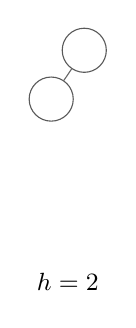
\begin{tikzpicture}[x=0.42cm,y=0.62cm,baseline=(current bounding box.north)]
\node[tn] (fb2x1) at (0,-1) {};
\node[tn] (fb2x2) at (1,0) {};
\draw[te] (fb2x2) -- (fb2x1);
\node[plab] at (0.5,-4.75) {$h = 2$};
\end{tikzpicture}\hspace{0.5cm}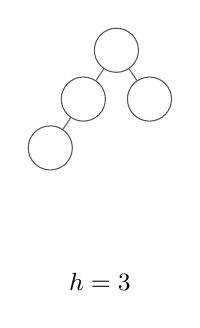
\begin{tikzpicture}[x=0.42cm,y=0.62cm,baseline=(current bounding box.north)]
\node[tn] (fb3x1) at (0,-2) {};
\node[tn] (fb3x2) at (1,-1) {};
\node[tn] (fb3x3) at (2,0) {};
\node[tn] (fb3x4) at (3,-1) {};
\draw[te] (fb3x3) -- (fb3x2);
\draw[te] (fb3x2) -- (fb3x1);
\draw[te] (fb3x3) -- (fb3x4);
\node[plab] at (1.5,-4.75) {$h = 3$};
\end{tikzpicture}\hspace{0.5cm}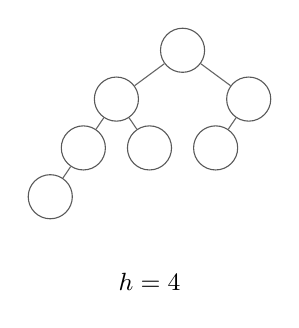
\begin{tikzpicture}[x=0.42cm,y=0.62cm,baseline=(current bounding box.north)]
\node[tn] (fb4x1) at (0,-3) {};
\node[tn] (fb4x2) at (1,-2) {};
\node[tn] (fb4x3) at (2,-1) {};
\node[tn] (fb4x4) at (3,-2) {};
\node[tn] (fb4x5) at (4,0) {};
\node[tn] (fb4x6) at (5,-2) {};
\node[tn] (fb4x7) at (6,-1) {};
\draw[te] (fb4x5) -- (fb4x3);
\draw[te] (fb4x3) -- (fb4x2);
\draw[te] (fb4x2) -- (fb4x1);
\draw[te] (fb4x3) -- (fb4x4);
\draw[te] (fb4x5) -- (fb4x7);
\draw[te] (fb4x7) -- (fb4x6);
\node[plab] at (3.0,-4.75) {$h = 4$};
\end{tikzpicture}\hspace{0.5cm}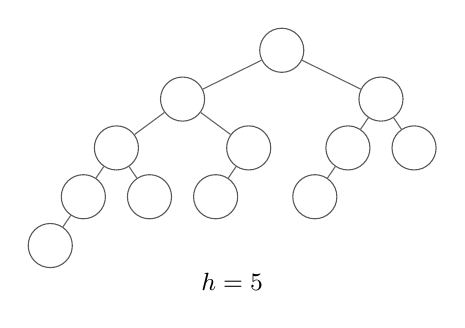
\begin{tikzpicture}[x=0.42cm,y=0.62cm,baseline=(current bounding box.north)]
\node[tn] (fb5x1) at (0,-4) {};
\node[tn] (fb5x2) at (1,-3) {};
\node[tn] (fb5x3) at (2,-2) {};
\node[tn] (fb5x4) at (3,-3) {};
\node[tn] (fb5x5) at (4,-1) {};
\node[tn] (fb5x6) at (5,-3) {};
\node[tn] (fb5x7) at (6,-2) {};
\node[tn] (fb5x8) at (7,0) {};
\node[tn] (fb5x9) at (8,-3) {};
\node[tn] (fb5x10) at (9,-2) {};
\node[tn] (fb5x11) at (10,-1) {};
\node[tn] (fb5x12) at (11,-2) {};
\draw[te] (fb5x8) -- (fb5x5);
\draw[te] (fb5x5) -- (fb5x3);
\draw[te] (fb5x3) -- (fb5x2);
\draw[te] (fb5x2) -- (fb5x1);
\draw[te] (fb5x3) -- (fb5x4);
\draw[te] (fb5x5) -- (fb5x7);
\draw[te] (fb5x7) -- (fb5x6);
\draw[te] (fb5x8) -- (fb5x11);
\draw[te] (fb5x11) -- (fb5x10);
\draw[te] (fb5x10) -- (fb5x9);
\draw[te] (fb5x11) -- (fb5x12);
\node[plab] at (5.5,-4.75) {$h = 5$};
\end{tikzpicture}
\diagcaption{節點最少的 AVL 樹，節點數依序是 $1, 2, 4, 7, 12$。 每一棵都是根加上
前兩棵。}
\label{fig:bal-fib}
\end{center}

先用一個粗略的估計看出它是對數：$N(h) = N(h-1) + N(h-2) + 1 > 2N(h-2)$，每往下兩
層節點數至少減半，從 $N(1) = 1$、$N(2) = 2$ 往上推，得到 $N(h) \ge 2^{(h-1)/2}$。 所
以 $n \ge 2^{(h-1)/2}$，$h \le 2\lg n + 1$。 精確的常數要用費氏數。 令 $F_1 = F_2 =
1$、$F_k = F_{k-1} + F_{k-2}$，$\varphi = (1 + \sqrt5)/2 \approx 1.618$ 是
$\varphi^2 = \varphi + 1$ 的正根。

\begin{theorem}
\label{thm:bal-avl-height}
(1) $N(h) = F_{h+2} - 1$。 (2) 有 $n$ 個節點的 AVL 樹，高度
\[
h \le \log_\varphi(n + 1) = \frac{\lg(n+1)}{\lg \varphi} < 1.4405 \lg(n+1).
\]
\end{theorem}

\begin{proof}
(1) 對 $h$ 歸納。 $N(0) + 1 = 1 = F_2$，$N(1) + 1 = 2 = F_3$。 $h \ge 2$ 時，遞迴式
兩邊加 $1$：
\[
N(h) + 1 = \bigl(N(h-1) + 1\bigr) + \bigl(N(h-2) + 1\bigr) = F_{h+1} + F_h = F_{h+2}.
\]

(2) 先證明 $F_k \ge \varphi^{k-2}$（$k \ge 1$）。 $F_1 = 1 > \varphi^{-1}$，
$F_2 = 1 = \varphi^0$。 $k \ge 3$ 時，由歸納假設
\[
F_k = F_{k-1} + F_{k-2} \ge \varphi^{k-3} + \varphi^{k-4} = \varphi^{k-4}(\varphi + 1)
= \varphi^{k-4} \varphi^2 = \varphi^{k-2}.
\]
高度 $h$ 的 AVL 樹有 $n \ge N(h)$ 個節點，所以
$n + 1 \ge N(h) + 1 = F_{h+2} \ge \varphi^h$，兩邊取 $\log_\varphi$ 得到
$h \le \log_\varphi(n+1)$。 $1 / \lg \varphi \approx 1.44042$。
\end{proof}

和最矮的可能 $\lceil \lg(n+1) \rceil$ 比，AVL 樹最壞只高了大約 $44\%$。 一百萬個節
點的二元樹至少高 $20$；AVL 樹最高 $28$（觀念題第 13 題）。

考卷上常問「$n$ 個節點的 AVL 樹最高可能是多少」。 做法是把 $N(h)$ 的表列到超過 $n$
為止，答案是滿足 $N(h) \le n$ 的最大 $h$。 例如 $n = 100$：$N(9) = 88 \le 100 <
143 = N(10)$，最高是 $9$；最矮是 $\lceil \lg 101 \rceil = 7$。 定理的上界
$\log_\varphi 101 \approx 9.59$ 只是估計，要算確切的值還是查表。

\subsection{插入：四種失衡和旋轉}
\label{sec:bal-avl-insert}

插入分三步。

\begin{enumerate}
\item 照第~9~章的方法，把新鍵插成葉節點。
\item 從新節點的父節點往根走，更新路上每個節點的高度和平衡因子。 只有這條路徑上的
節點，子樹的內容變了，其他節點的高度不會變。
\item 在這條路上找\textbf{第一個}（離新節點最近的）平衡因子變成 $\pm 2$ 的節點，
叫它 $A$。 從 $A$ 往新節點走兩步，依照這兩步的方向分成四種情況，各用一種旋轉修
好。 沒有任何節點變成 $\pm 2$，就不用旋轉。
\end{enumerate}

\begin{center}
\begin{tabular}{cll}
\toprule
類型 & 新節點在哪裡 & 修正 \\
\midrule
LL & $A$ 的左子節點的左子樹 & 對 $A$ 右旋 \\
RR & $A$ 的右子節點的右子樹 & 對 $A$ 左旋 \\
LR & $A$ 的左子節點的右子樹 & 先對 $A$ 的左子節點左旋，再對 $A$ 右旋 \\
RL & $A$ 的右子節點的左子樹 & 先對 $A$ 的右子節點右旋，再對 $A$ 左旋 \\
\bottomrule
\end{tabular}
\end{center}

LL、RR 叫\textbf{單旋轉}，LR、RL 叫\textbf{雙旋轉}。 RR、RL 是 LL、LR 左右對調，下
面只分析 LL 和 LR。

\textbf{LL}。 設 $B$ 是 $A$ 的左子節點。 插入後 $A$ 是 $+2$，$B$ 的平衡因子只能是
$+1$：如果是 $0$，表示 $B$ 的高度沒有因為這次插入而增加，$A$ 就不會失衡；如果是
$\pm 2$，最近的失衡節點就是 $B$ 而不是 $A$。 所以插入前 $B$ 是 $0$，兩棵子樹
$T_1$、$T_2$ 同高，設為 $k$；$A$ 插入前是 $+1$，右子樹 $T_3$ 的高度是 $k$。 新節
點讓 $T_1$ 變成 $k + 1$。 對 $A$ 右旋之後，$A$ 的兩棵子樹是 $T_2$、$T_3$，都是
$k$；$B$ 的兩棵子樹是 $T_1$ 和 $A$，都是 $k + 1$。 兩個節點都變成 $0$，這一段的
高度是 $k + 2$，和插入\textbf{前}一樣。

\textbf{LR}。 新節點在 $B$ 的右子樹裡，設 $C$ 是 $B$ 的右子節點，$C$ 的兩棵子樹是
$T_2$、$T_3$。 同樣的理由，插入前 $B$、$C$ 都是 $0$，$T_1$ 高 $k$，$T_2$、$T_3$ 高
$k - 1$，$T_4$（$A$ 的右子樹）高 $k$。 新節點讓 $T_2$ 或 $T_3$ 其中一棵變成 $k$。
這時對 $A$ 右旋沒有用：$T_2$、$T_3$ 會跟著 $C$ 一起掛到 $A$ 底下，左邊變成右邊太
高。 正確的做法是讓 $C$ 升兩層：先對 $B$ 左旋（變成 LL 的樣子），再對 $A$ 右旋。
結果 $C$ 是根，左邊是 $B$（子樹 $T_1$、$T_2$），右邊是 $A$（子樹 $T_3$、$T_4$），
$B$、$A$ 的高度都是 $k + 1$，$C$ 是 $k + 2$，也和插入前一樣。

\begin{center}
\begin{tikzpicture}[x=0.8cm, y=0.82cm]
% LL 之前
\node[tn, tnA] (A) at (0,0) {$A$};
\node[tn] (B) at (-1.1,-1) {$B$};
\draw[te] (A) -- (B); \draw[te] (A) -- (1.0,-1.0); \draw[te] (B) -- (-1.7,-2); \draw[te] (B) -- (-0.5,-2);
\subtri[1.25]{-1.7}{-2}{$T_1$}
\subtri{-0.5}{-2}{$T_2$}
\subtri{1.0}{-1}{$T_3$}
\node[bfl] at (A.north east) {$+2$}; \node[bfl] at (B.north east) {$+1$};
\node[font=\scriptsize] at (-1.7,-3.5) {$k+1$};
\node[font=\scriptsize] at (-0.5,-3.15) {$k$};
\node[font=\scriptsize] at (1.0,-2.15) {$k$};
\fill[coreStroke] (-1.7,-3.15) circle (2.5pt);
\draw[tarr] (1.9,-1.2) -- node[above, font=\small] {右旋 $A$} (3.4,-1.2);
\begin{scope}[xshift=4.9cm]
\node[tn] (B2) at (0,0) {$B$};
\node[tn] (A2) at (1.1,-1) {$A$};
\draw[te] (B2) -- (A2); \draw[te] (B2) -- (-1.0,-1.0); \draw[te] (A2) -- (0.5,-2); \draw[te] (A2) -- (1.7,-2);
\subtri[1.25]{-1.0}{-1}{$T_1$}
\subtri{0.5}{-2}{$T_2$}
\subtri{1.7}{-2}{$T_3$}
\node[bfl] at (A2.north east) {$0$}; \node[bfl] at (B2.north east) {$0$};
\fill[coreStroke] (-1.0,-2.15) circle (2.5pt);
\end{scope}
\end{tikzpicture}\\*[0.6em]
\begin{tikzpicture}[x=0.8cm, y=0.82cm]
% LR 之前
\node[tn, tnA] (A) at (0,0) {$A$};
\node[tn] (B) at (-1.3,-1) {$B$};
\node[tn] (C) at (-0.6,-2) {$C$};
\draw[te] (A) -- (B); \draw[te] (A) -- (1.0,-1.0); \draw[te] (B) -- (-2.0,-2); \draw[te] (B) -- (C);
\draw[te] (C) -- (-1.1,-3); \draw[te] (C) -- (-0.1,-3);
\subtri[1.6]{-2.0}{-2}{$T_1$}
\subtri[0.9]{-1.1}{-3}{$T_2$}
\subtri[0.9]{-0.1}{-3}{$T_3$}
\subtri[1.6]{1.0}{-1}{$T_4$}
\node[bfl] at (A.north east) {$+2$}; \node[bfl] at (B.north east) {$-1$};
\node[font=\scriptsize] at (-2.0,-3.85) {$k$};
\node[font=\scriptsize] at (1.0,-2.85) {$k$};
\node[font=\scriptsize, align=center] at (-0.6,-4.35) {其中一棵 $k$，\\ 另一棵 $k-1$};
\draw[tarr] (1.9,-1.4) -- node[above, font=\small] {左旋 $B$} node[below, font=\small] {再右旋 $A$} (3.6,-1.4);
\begin{scope}[xshift=5.6cm]
\node[tn] (C2) at (0,0) {$C$};
\node[tn] (B2) at (-1.1,-1) {$B$};
\node[tn] (A2) at (1.1,-1) {$A$};
\draw[te] (C2) -- (B2); \draw[te] (C2) -- (A2);
\draw[te] (B2) -- (-1.6,-2); \draw[te] (B2) -- (-0.6,-2); \draw[te] (A2) -- (0.6,-2); \draw[te] (A2) -- (1.6,-2);
\subtri[1.6]{-1.6}{-2}{$T_1$}
\subtri[0.9]{-0.6}{-2}{$T_2$}
\subtri[0.9]{0.6}{-2}{$T_3$}
\subtri[1.6]{1.6}{-2}{$T_4$}
\node[bfl] at (C2.north east) {$0$};
\end{scope}
\end{tikzpicture}
\diagcaption{上：LL，藍點是新節點，落在 $T_1$。 下：LR，新節點落在 $T_2$ 或
$T_3$（$k = 0$ 時 $C$ 自己就是新節點）。 兩種修完之後，這一段的高度都回到插入
前的 $k + 2$。}
\label{fig:bal-ll-lr}
\end{center}

兩種情況修完，這一段的高度都和插入前一樣，所以 $A$ 上面的祖先，高度和平衡因子都
回到插入前的樣子，不會再失衡。 這證明了：

\begin{theorem}
\label{thm:bal-avl-insert}
AVL 樹插入一個鍵，最多做一次單旋轉或一次雙旋轉（也就是最多兩次旋轉）。 整個插入
的時間是 $O(\lg n)$。
\end{theorem}

雙旋轉之後 $A$、$B$ 的平衡因子是多少，要看新節點落在 $T_2$ 還是 $T_3$，觀念題第 5
題會整理。 程式不用記這張表：每個節點存高度，旋轉後重算就好。

\begin{pseudo}[label=alg:bal-avl-insert]{AVL 樹的插入，回傳新的根}
\Function{AVL-Insert}{$t, k$}
    \If{$t = \NIL$}
        \State \Return 新節點（$\mathit{key} = k$、$\mathit{height} = 1$、兩個子指標都是 \NIL）
    \EndIf
    \If{$k < t.\mathit{key}$}
        \State $t.\mathit{left} \gets \Call{AVL-Insert}{t.\mathit{left}, k}$
    \ElsIf{$k > t.\mathit{key}$}
        \State $t.\mathit{right} \gets \Call{AVL-Insert}{t.\mathit{right}, k}$
    \Else
        \State \Return $t$ \Comment{已經在樹裡}
    \EndIf
    \State $t.\mathit{height} \gets 1 + \max(h(t.\mathit{left}), h(t.\mathit{right}))$
    \State \Return \Call{Rebalance}{$t$}
\EndFunction
\end{pseudo}

\begin{pseudo}[label=alg:bal-rebalance]{檢查 $t$ 是否失衡，失衡就旋轉}
\Function{Rebalance}{$t$}
    \If{$\mathrm{BF}(t) = 2$}
        \If{$\mathrm{BF}(t.\mathit{left}) < 0$} \Comment{LR：先轉成 LL}
            \State $t.\mathit{left} \gets \Call{Rotate-Left}{t.\mathit{left}}$
        \EndIf
        \State \Return \Call{Rotate-Right}{$t$}
    \ElsIf{$\mathrm{BF}(t) = -2$}
        \If{$\mathrm{BF}(t.\mathit{right}) > 0$} \Comment{RL：先轉成 RR}
            \State $t.\mathit{right} \gets \Call{Rotate-Right}{t.\mathit{right}}$
        \EndIf
        \State \Return \Call{Rotate-Left}{$t$}
    \EndIf
    \State \Return $t$
\EndFunction
\end{pseudo}

$h(\NIL) = 0$。 這裡的 \proc{Rotate-Right}、\proc{Rotate-Left} 是虛擬碼~\ref{alg:bal-rotate-right}
加上最後兩步：先重算降下去的節點的高度，再重算升上來的節點（它的高度要用到前者）。

遞迴版本在回程時對路徑上的每個節點都呼叫 \proc{Rebalance}，第一個失衡的節點就是
最深的那個，也就是上面說的 $A$。 修完之後高度回到插入前，上面的節點自然不會再旋
轉。 \proc{Rebalance} 第 3 行用的是嚴格的 $< 0$：插入時 $A$ 的子節點不會是 $0$，
但刪除時會，那時必須做單旋轉（第~\ref{sec:bal-avl-delete}~節）。

\subsection{手算追蹤：依序登錄會員卡}
\label{sec:bal-avl-trace}

健身房把十張紙本會員卡登錄進系統，依收到卡片的順序插入 AVL 樹，編號是
\[
52,\ 41,\ 16,\ 34,\ 89,\ 94,\ 64,\ 46,\ 56,\ 58 .
\]
下面每張圖的節點右上方是平衡因子，藍底是剛插入的節點，橘框是第一個失衡的節點
$A$。 沒有引起旋轉的插入合併成一張。

\begin{center}
\begin{tikzpicture}[x=0.5cm,y=0.72cm,baseline=(current bounding box.north)]
\node[tn] (aia41) at (0,-1) {41};
\node[tn] (aia52) at (1,0) {52};
\draw[te] (aia52) -- (aia41);
\node[bfl] at (aia41.north east) {$0$};
\node[bfl] at (aia52.north east) {$+1$};
\node[plab] at (0.5,-2.75) {(a) 插入 52、41};
\end{tikzpicture}\hspace{0.8cm}\begin{tikzpicture}[x=0.5cm,y=0.72cm,baseline=(current bounding box.north)]
\node[tn,tnN] (aib16) at (0,-2) {16};
\node[tn] (aib41) at (1,-1) {41};
\node[tn,tnA] (aib52) at (2,0) {52};
\draw[te] (aib52) -- (aib41);
\draw[te] (aib41) -- (aib16);
\node[bfl] at (aib16.north east) {$0$};
\node[bfl] at (aib41.north east) {$+1$};
\node[bfl] at (aib52.north east) {$+2$};
\node[plab] at (1.0,-2.75) {(b) 插入 16：LL};
\end{tikzpicture}\hspace{0.8cm}\begin{tikzpicture}[x=0.5cm,y=0.72cm,baseline=(current bounding box.north)]
\node[tn] (aic16) at (0,-1) {16};
\node[tn] (aic41) at (1,0) {41};
\node[tn] (aic52) at (2,-1) {52};
\draw[te] (aic41) -- (aic16);
\draw[te] (aic41) -- (aic52);
\node[bfl] at (aic16.north east) {$0$};
\node[bfl] at (aic41.north east) {$0$};
\node[bfl] at (aic52.north east) {$0$};
\node[plab] at (1.0,-2.75) {(c) 右旋之後};
\end{tikzpicture}\\*[0.6em]
\begin{tikzpicture}[x=0.5cm,y=0.72cm,baseline=(current bounding box.north)]
\node[tn] (aid16) at (0,-1) {16};
\node[tn] (aid34) at (1,-2) {34};
\node[tn] (aid41) at (2,0) {41};
\node[tn] (aid52) at (3,-1) {52};
\node[tn] (aid89) at (4,-2) {89};
\draw[te] (aid41) -- (aid16);
\draw[te] (aid16) -- (aid34);
\draw[te] (aid41) -- (aid52);
\draw[te] (aid52) -- (aid89);
\node[bfl] at (aid16.north east) {$-1$};
\node[bfl] at (aid34.north east) {$0$};
\node[bfl] at (aid41.north east) {$0$};
\node[bfl] at (aid52.north east) {$-1$};
\node[bfl] at (aid89.north east) {$0$};
\node[plab] at (2.0,-3.75) {(d) 插入 34、89};
\end{tikzpicture}\hspace{0.6cm}\begin{tikzpicture}[x=0.5cm,y=0.72cm,baseline=(current bounding box.north)]
\node[tn] (aie16) at (0,-1) {16};
\node[tn] (aie34) at (1,-2) {34};
\node[tn] (aie41) at (2,0) {41};
\node[tn,tnA] (aie52) at (3,-1) {52};
\node[tn] (aie89) at (4,-2) {89};
\node[tn,tnN] (aie94) at (5,-3) {94};
\draw[te] (aie41) -- (aie16);
\draw[te] (aie16) -- (aie34);
\draw[te] (aie41) -- (aie52);
\draw[te] (aie52) -- (aie89);
\draw[te] (aie89) -- (aie94);
\node[bfl] at (aie16.north east) {$-1$};
\node[bfl] at (aie34.north east) {$0$};
\node[bfl] at (aie41.north east) {$-1$};
\node[bfl] at (aie52.north east) {$-2$};
\node[bfl] at (aie89.north east) {$-1$};
\node[bfl] at (aie94.north east) {$0$};
\node[plab] at (2.5,-3.75) {(e) 插入 94：RR};
\end{tikzpicture}\hspace{0.6cm}\begin{tikzpicture}[x=0.5cm,y=0.72cm,baseline=(current bounding box.north)]
\node[tn] (aif16) at (0,-1) {16};
\node[tn] (aif34) at (1,-2) {34};
\node[tn] (aif41) at (2,0) {41};
\node[tn] (aif52) at (3,-2) {52};
\node[tn] (aif89) at (4,-1) {89};
\node[tn] (aif94) at (5,-2) {94};
\draw[te] (aif41) -- (aif16);
\draw[te] (aif16) -- (aif34);
\draw[te] (aif41) -- (aif89);
\draw[te] (aif89) -- (aif52);
\draw[te] (aif89) -- (aif94);
\node[bfl] at (aif16.north east) {$-1$};
\node[bfl] at (aif34.north east) {$0$};
\node[bfl] at (aif41.north east) {$0$};
\node[bfl] at (aif52.north east) {$0$};
\node[bfl] at (aif89.north east) {$0$};
\node[bfl] at (aif94.north east) {$0$};
\node[plab] at (2.5,-3.75) {(f) 左旋之後};
\end{tikzpicture}
\diagcaption{插入 $52$ 到 $94$。 (b) 從 $16$ 往上，$41$ 變 $+1$，$52$ 變 $+2$，兩步
都往左，是 LL。 (e) $89$ 變 $-1$，$52$ 變 $-2$，兩步都往右，是 RR。 根 $41$ 是 $-1$，沒有失衡。}
\label{fig:bal-avl-trace1}
\end{center}

插入 $64$、$46$ 都沒有失衡：$64$ 讓 $52$ 變 $-1$、$89$ 變 $+1$、$41$ 變 $-1$；
$46$ 讓 $52$ 回到 $0$，$52$ 的高度沒變，再往上的節點都不受影響。

\begin{center}
\begin{tikzpicture}[x=0.5cm,y=0.72cm,baseline=(current bounding box.north)]
\node[tn] (aig16) at (0,-1) {16};
\node[tn] (aig34) at (1,-2) {34};
\node[tn] (aig41) at (2,0) {41};
\node[tn] (aig46) at (3,-3) {46};
\node[tn] (aig52) at (4,-2) {52};
\node[tn] (aig64) at (5,-3) {64};
\node[tn] (aig89) at (6,-1) {89};
\node[tn] (aig94) at (7,-2) {94};
\draw[te] (aig41) -- (aig16);
\draw[te] (aig16) -- (aig34);
\draw[te] (aig41) -- (aig89);
\draw[te] (aig89) -- (aig52);
\draw[te] (aig52) -- (aig46);
\draw[te] (aig52) -- (aig64);
\draw[te] (aig89) -- (aig94);
\node[bfl] at (aig16.north east) {$-1$};
\node[bfl] at (aig34.north east) {$0$};
\node[bfl] at (aig41.north east) {$-1$};
\node[bfl] at (aig46.north east) {$0$};
\node[bfl] at (aig52.north east) {$0$};
\node[bfl] at (aig64.north east) {$0$};
\node[bfl] at (aig89.north east) {$+1$};
\node[bfl] at (aig94.north east) {$0$};
\node[plab] at (3.5,-4.75) {(g) 插入 64、46};
\end{tikzpicture}\hspace{0.4cm}\begin{tikzpicture}[x=0.5cm,y=0.72cm,baseline=(current bounding box.north)]
\node[tn] (aih16) at (0,-1) {16};
\node[tn] (aih34) at (1,-2) {34};
\node[tn] (aih41) at (2,0) {41};
\node[tn] (aih46) at (3,-3) {46};
\node[tn] (aih52) at (4,-2) {52};
\node[tn,tnN] (aih56) at (5,-4) {56};
\node[tn] (aih64) at (6,-3) {64};
\node[tn,tnA] (aih89) at (7,-1) {89};
\node[tn] (aih94) at (8,-2) {94};
\draw[te] (aih41) -- (aih16);
\draw[te] (aih16) -- (aih34);
\draw[te] (aih41) -- (aih89);
\draw[te] (aih89) -- (aih52);
\draw[te] (aih52) -- (aih46);
\draw[te] (aih52) -- (aih64);
\draw[te] (aih64) -- (aih56);
\draw[te] (aih89) -- (aih94);
\node[bfl] at (aih16.north east) {$-1$};
\node[bfl] at (aih34.north east) {$0$};
\node[bfl] at (aih41.north east) {$-2$};
\node[bfl] at (aih46.north east) {$0$};
\node[bfl] at (aih52.north east) {$-1$};
\node[bfl] at (aih56.north east) {$0$};
\node[bfl] at (aih64.north east) {$+1$};
\node[bfl] at (aih89.north east) {$+2$};
\node[bfl] at (aih94.north east) {$0$};
\node[plab] at (4.0,-4.75) {(h) 插入 56：LR};
\end{tikzpicture}\hspace{0.4cm}\begin{tikzpicture}[x=0.5cm,y=0.72cm,baseline=(current bounding box.north)]
\node[tn] (aii16) at (0,-1) {16};
\node[tn] (aii34) at (1,-2) {34};
\node[tn] (aii41) at (2,0) {41};
\node[tn] (aii46) at (3,-3) {46};
\node[tn] (aii52) at (4,-2) {52};
\node[tn] (aii56) at (5,-3) {56};
\node[tn] (aii64) at (6,-1) {64};
\node[tn] (aii89) at (7,-2) {89};
\node[tn] (aii94) at (8,-3) {94};
\draw[te] (aii41) -- (aii16);
\draw[te] (aii16) -- (aii34);
\draw[te] (aii41) -- (aii64);
\draw[te] (aii64) -- (aii52);
\draw[te] (aii52) -- (aii46);
\draw[te] (aii52) -- (aii56);
\draw[te] (aii64) -- (aii89);
\draw[te] (aii89) -- (aii94);
\node[bfl] at (aii16.north east) {$-1$};
\node[bfl] at (aii34.north east) {$0$};
\node[bfl] at (aii41.north east) {$-1$};
\node[bfl] at (aii46.north east) {$0$};
\node[bfl] at (aii52.north east) {$0$};
\node[bfl] at (aii56.north east) {$0$};
\node[bfl] at (aii64.north east) {$0$};
\node[bfl] at (aii89.north east) {$-1$};
\node[bfl] at (aii94.north east) {$0$};
\node[plab] at (4.0,-4.75) {(i) 雙旋轉之後};
\end{tikzpicture}
\diagcaption{插入 $56$。 從 $56$ 往上：$64$ 變 $+1$，$52$ 變 $-1$，$89$ 變 $+2$。 從
$89$ 往 $56$ 先左（$52$）再右（$64$），是 LR：先對 $52$ 左旋，再對 $89$ 右旋，
$64$ 升到這一段的根。 $64$ 原本的左子節點 $56$ 換到 $52$ 的右邊。}
\label{fig:bal-avl-trace2}
\end{center}

\begin{center}
\begin{tikzpicture}[x=0.5cm,y=0.72cm,baseline=(current bounding box.north)]
\node[tn] (aij16) at (0,-1) {16};
\node[tn] (aij34) at (1,-2) {34};
\node[tn,tnA] (aij41) at (2,0) {41};
\node[tn] (aij46) at (3,-3) {46};
\node[tn] (aij52) at (4,-2) {52};
\node[tn] (aij56) at (5,-3) {56};
\node[tn,tnN] (aij58) at (6,-4) {58};
\node[tn] (aij64) at (7,-1) {64};
\node[tn] (aij89) at (8,-2) {89};
\node[tn] (aij94) at (9,-3) {94};
\draw[te] (aij41) -- (aij16);
\draw[te] (aij16) -- (aij34);
\draw[te] (aij41) -- (aij64);
\draw[te] (aij64) -- (aij52);
\draw[te] (aij52) -- (aij46);
\draw[te] (aij52) -- (aij56);
\draw[te] (aij56) -- (aij58);
\draw[te] (aij64) -- (aij89);
\draw[te] (aij89) -- (aij94);
\node[bfl] at (aij16.north east) {$-1$};
\node[bfl] at (aij34.north east) {$0$};
\node[bfl] at (aij41.north east) {$-2$};
\node[bfl] at (aij46.north east) {$0$};
\node[bfl] at (aij52.north east) {$-1$};
\node[bfl] at (aij56.north east) {$-1$};
\node[bfl] at (aij58.north east) {$0$};
\node[bfl] at (aij64.north east) {$+1$};
\node[bfl] at (aij89.north east) {$-1$};
\node[bfl] at (aij94.north east) {$0$};
\node[plab] at (4.5,-4.75) {(j) 插入 58：RL};
\end{tikzpicture}\hspace{1.0cm}\begin{tikzpicture}[x=0.5cm,y=0.72cm,baseline=(current bounding box.north)]
\node[tn] (aik16) at (0,-2) {16};
\node[tn] (aik34) at (1,-3) {34};
\node[tn] (aik41) at (2,-1) {41};
\node[tn] (aik46) at (3,-2) {46};
\node[tn] (aik52) at (4,0) {52};
\node[tn] (aik56) at (5,-2) {56};
\node[tn] (aik58) at (6,-3) {58};
\node[tn] (aik64) at (7,-1) {64};
\node[tn] (aik89) at (8,-2) {89};
\node[tn] (aik94) at (9,-3) {94};
\draw[te] (aik52) -- (aik41);
\draw[te] (aik41) -- (aik16);
\draw[te] (aik16) -- (aik34);
\draw[te] (aik41) -- (aik46);
\draw[te] (aik52) -- (aik64);
\draw[te] (aik64) -- (aik56);
\draw[te] (aik56) -- (aik58);
\draw[te] (aik64) -- (aik89);
\draw[te] (aik89) -- (aik94);
\node[bfl] at (aik16.north east) {$-1$};
\node[bfl] at (aik34.north east) {$0$};
\node[bfl] at (aik41.north east) {$+1$};
\node[bfl] at (aik46.north east) {$0$};
\node[bfl] at (aik52.north east) {$0$};
\node[bfl] at (aik56.north east) {$-1$};
\node[bfl] at (aik58.north east) {$0$};
\node[bfl] at (aik64.north east) {$0$};
\node[bfl] at (aik89.north east) {$-1$};
\node[bfl] at (aik94.north east) {$0$};
\node[plab] at (4.5,-4.75) {(k) 雙旋轉之後};
\end{tikzpicture}
\diagcaption{插入 $58$。 $56$ 變 $-1$，$52$ 變 $-1$，$64$ 變 $+1$，根 $41$ 變
$-2$。 從 $41$ 先右（$64$）再左（$52$），是 RL：先對 $64$ 右旋，再對 $41$ 左旋，
$52$ 升到根。 $52$ 原本的左子樹 $46$ 接到 $41$ 的右邊，右子樹 $56$ 接到 $64$ 的
左邊。}
\label{fig:bal-avl-trace3}
\end{center}

整理成表：

\begin{center}
\begin{tabular}{cccl}
\toprule
插入 & 失衡節點 $A$ & 類型 & 修完後這一段的根 \\
\midrule
16 & 52 & LL & 41 \\
94 & 52 & RR & 89 \\
56 & 89 & LR & 64 \\
58 & 41 & RL & 52 \\
\bottomrule
\end{tabular}
\end{center}

圖~\ref{fig:bal-avl-trace3}(k) 的最後一步最容易畫錯。 雙旋轉的結果可以不畫中間那一
步，直接寫：$A$、$B$、$C$ 三個節點依鍵的大小排好，中間的 $C$ 當根，小的當左子節點，
大的當右子節點；原本掛在這三個節點底下的四棵子樹，依中序順序從左到右接上去。 這裡
三個節點是 $41 < 52 < 64$，四棵子樹依序是 $\{16, 34\}$、$\{46\}$、$\{56, 58\}$、
$\{89, 94\}$。 單旋轉也可以這樣想，只是三個節點是 $A$、$B$ 和 $B$ 往同一邊的子節點。

\begin{examnote}
AVL 的追蹤題，每次旋轉都要畫出旋轉後的整棵樹，並寫出失衡的節點和類型（LL、RR、
LR、RL）。 沒有旋轉的插入可以幾個合併成一張。 判斷類型時，從\textbf{最靠近新節
點}的失衡節點往下看兩步，不是從根看。 最後檢查一次：中序是不是由小到大，每個節點
的平衡因子是不是都在 $-1$ 到 $1$。
\end{examnote}

\subsection{C 程式}
\label{sec:bal-avl-c}

C 程式照虛擬碼~\ref{alg:bal-avl-insert}、\ref{alg:bal-rebalance} 寫。 每個節點多存
一個 \texttt{height}，平衡因子要用時再算。 遞迴函式回傳這棵子樹新的根，呼叫的地方
寫 \texttt{t->left = avl\_insert(t->left, key, rot)}，旋轉換了根也接得回去。
\texttt{Rotation} 結構只是用來把旋轉的類型和位置帶回 \texttt{main} 印出來。

\begin{cbookrecap}[第~14~章 14.5 節、第~15~章、第~19~章 19.10、19.15、19.17 節]
\texttt{t->left} 是 \texttt{(*t).left} 的簡寫，\texttt{t} 是指向結構的指標。 遞迴
函式回傳 \texttt{Node *}，呼叫端把回傳值接回原本的指標，是串列和樹最常見的寫法：
不用傳指標的指標，空樹的情況（\texttt{t == NULL}）也不用另外處理。 釋放整棵樹要
先釋放兩棵子樹，最後才釋放自己（後序），順序反過來就會讀到已經釋放的記憶體。
\end{cbookrecap}

\begin{example}[label=ex:bal-avl-insert]{c}{(avl\_insert.c) AVL 樹的插入}
#include <stdio.h>
#include <stdlib.h>

typedef struct Node {
    int key;
    int height;                 // 這棵子樹的高度，只有一個節點時是 1
    struct Node *left, *right;
} Node;

typedef struct {
    const char *type;           // "LL"、"RR"、"LR"、"RL"；沒有旋轉時是 NULL
    int at;                     // 失衡節點的鍵
} Rotation;

static int height(const Node *t)
{
    return t == NULL ? 0 : t->height;
}

static void update(Node *t)
{
    int hl = height(t->left), hr = height(t->right);
    t->height = 1 + (hl > hr ? hl : hr);
}

static int balance(const Node *t)       // 平衡因子：左高減右高
{
    return height(t->left) - height(t->right);
}

static Node *rotate_right(Node *a)      // a 的左子節點 b 轉上來
{
    Node *b = a->left;
    a->left = b->right;
    b->right = a;
    update(a);                          // a 現在在 b 下面，先更新 a
    update(b);
    return b;
}

static Node *rotate_left(Node *a)       // a 的右子節點 b 轉上來
{
    Node *b = a->right;
    a->right = b->left;
    b->left = a;
    update(a);
    update(b);
    return b;
}

// 檢查 t 是否失衡；失衡就旋轉，回傳這棵子樹新的根。
static Node *rebalance(Node *t, Rotation *rot)
{
    int b = balance(t);
    if (b == 2) {                               // 左邊太高
        rot->at = t->key;
        if (balance(t->left) < 0) {
            rot->type = "LR";
            t->left = rotate_left(t->left);
        } else {
            rot->type = "LL";
        }
        return rotate_right(t);
    }
    if (b == -2) {                              // 右邊太高
        rot->at = t->key;
        if (balance(t->right) > 0) {
            rot->type = "RL";
            t->right = rotate_right(t->right);
        } else {
            rot->type = "RR";
        }
        return rotate_left(t);
    }
    return t;
}

// 把 key 插進以 t 為根的 AVL 樹，回傳新的根。key 已經在樹裡就不插。
Node *avl_insert(Node *t, int key, Rotation *rot)
{
    if (t == NULL) {
        Node *x = malloc(sizeof *x);
        if (x == NULL) {
            exit(1);
        }
        x->key = key;
        x->height = 1;
        x->left = x->right = NULL;
        return x;
    }
    if (key < t->key) {
        t->left = avl_insert(t->left, key, rot);
    } else if (key > t->key) {
        t->right = avl_insert(t->right, key, rot);
    } else {
        return t;
    }
    update(t);
    return rebalance(t, rot);
}

// 用「根(左子樹,右子樹)」的格式印出，空的子樹印成 .
void print_tree(const Node *t)
{
    if (t == NULL) {
        putchar('.');
        return;
    }
    printf("%d", t->key);
    if (t->left != NULL || t->right != NULL) {
        putchar('(');
        print_tree(t->left);
        putchar(',');
        print_tree(t->right);
        putchar(')');
    }
}

void free_tree(Node *t)
{
    if (t != NULL) {
        free_tree(t->left);
        free_tree(t->right);
        free(t);
    }
}

int main(void)
{
    int keys[] = {52, 41, 16, 34, 89, 94, 64, 46, 56, 58};
    int n = sizeof keys / sizeof keys[0];
    Node *root = NULL;
    for (int i = 0; i < n; i++) {
        Rotation rot = {NULL, 0};
        root = avl_insert(root, keys[i], &rot);
        printf("insert %d: ", keys[i]);
        if (rot.type != NULL) {
            printf("%s at %d, ", rot.type, rot.at);
        }
        print_tree(root);
        putchar('\n');
    }
    printf("height = %d\n", height(root));
    free_tree(root);

    // 會員編號由小到大插入：1, 2, ..., m
    for (int m = 1000; m <= 1000000; m *= 10) {
        Rotation rot = {NULL, 0};
        root = NULL;
        for (int k = 1; k <= m; k++) {
            root = avl_insert(root, k, &rot);
        }
        int lg = 0;                     // lg = ceil(lg(m + 1))，m 個節點的最小高度
        while ((1L << lg) < m + 1) {
            lg++;
        }
        printf("sorted m = %d: height = %d, minimum = %d\n", m, height(root), lg);
        free_tree(root);
    }
    return 0;
}
\end{example}
\iosample{}{insert 52: 52 \\ insert 41: 52(41,.) \\ insert 16: LL at 52, 41(16,52) \\ insert 34: 41(16(.,34),52) \\ insert 89: 41(16(.,34),52(.,89)) \\ insert 94: RR at 52, 41(16(.,34),89(52,94)) \\ insert 64: 41(16(.,34),89(52(.,64),94)) \\ insert 46: 41(16(.,34),89(52(46,64),94)) \\ insert 56: LR at 89, 41(16(.,34),64(52(46,56),89(.,94))) \\ insert 58: RL at 41, 52(41(16(.,34),46),64(56(.,58),89(.,94))) \\ height = 4 \\ sorted m = 1000: height = 10, minimum = 10 \\ sorted m = 10000: height = 14, minimum = 14 \\ sorted m = 100000: height = 17, minimum = 17 \\ sorted m = 1000000: height = 20, minimum = 20}

前十行和第~\ref{sec:bal-avl-trace}~節的圖一致。 後四行把 $1, 2, \ldots, m$ 依序插
入：普通的二元搜尋樹會長成高度 $m$ 的鏈，AVL 樹的高度剛好是最小可能值
$\lceil \lg(m+1) \rceil$。 依序插入時，需要旋轉的都是 RR，最後得到的樹非常整齊；一般的輸入不會這麼好，但高度不會超過定理~\ref{thm:bal-avl-height} 的上界。

\texttt{rotate\_right} 裡先 \texttt{update(a)} 再 \texttt{update(b)}：旋轉後 \texttt{a}
是 \texttt{b} 的子節點，\texttt{b} 的高度要用到 \texttt{a} 新的高度。 這兩行對調，
\texttt{b} 會用舊的高度算，之後的平衡因子全部算錯，而且不會當掉，很難查。

\subsection{刪除}
\label{sec:bal-avl-delete}

刪除也分三步。

\begin{enumerate}
\item 照第~9~章的方法刪除。 要刪的節點有兩個子節點時，用右子樹最小的節點（中序的
\textbf{後繼}）的鍵取代它，再去右子樹刪掉那個後繼。 真正被拿掉的節點最多只有一個
子節點。
\item 從被拿掉的節點的父節點往根走，更新高度和平衡因子。
\item 遇到平衡因子變成 $\pm 2$ 的節點 $A$，就旋轉。 \textbf{旋轉之後要繼續往上檢查}。
\end{enumerate}

刪除和插入不一樣的地方在第 3 步。 假設 $A$ 變成 $+2$（右邊少了一層），$B$ 是 $A$
的左子節點，也就是比較高的那一邊。 插入時 $B$ 一定是 $\pm 1$，刪除時 $B$ 可能是
$0$，因為 $B$ 這邊沒有動過。 三種情況：

\begin{center}
\begin{tabular}{cclc}
\toprule
$\mathrm{BF}(B)$ & 有些書的名稱 & 修正 & 這一段的高度 \\
\midrule
$+1$ & R1 & 對 $A$ 右旋（同 LL） & 少 $1$，要繼續往上 \\
$0$ & R0 & 對 $A$ 右旋（同 LL） & 不變，可以停 \\
$-1$ & R$-1$ & 先左旋 $B$，再右旋 $A$（同 LR） & 少 $1$，要繼續往上 \\
\bottomrule
\end{tabular}
\end{center}

名稱裡的 R 表示刪除發生在 $A$ 的右子樹，數字是 $\mathrm{BF}(B)$。 $A$ 變成 $-2$ 的
情況左右對調，叫 L0、L1、L$-1$，修正是 RR 或 RL。

$\mathrm{BF}(B) = 0$ 為什麼只能單旋轉、而且高度不變？ 設刪除後 $A$ 的右子樹高
$k$，$B$ 的兩棵子樹都高 $k + 1$，$A$ 原本高 $k + 3$。 對 $A$ 右旋後，$A$ 的子樹是
$B$ 原本的右子樹（$k + 1$）和 $A$ 的右子樹（$k$），$A$ 高 $k + 2$、平衡因子 $+1$；
$B$ 的子樹是 $k + 1$ 和 $k + 2$，平衡因子 $-1$，高度 $k + 3$，和刪除前一樣。 如果
這時誤用雙旋轉，$C$（$B$ 的右子節點，高 $k + 1$）升上來，$B$ 降成 $C$ 的左子節點：
$B$ 的左子樹（$k + 1$）留在 $B$ 底下，右邊換成 $C$ 原本的左子樹，只有 $k$ 或 $k - 1$
高；是 $k - 1$ 時，$B$ 的平衡因子變成 $+2$，又失衡了。 這就是 \proc{Rebalance} 第 3 行要用
$< 0$ 的原因：$\mathrm{BF}(B) = 0$ 時走單旋轉。

$\mathrm{BF}(B) = \pm 1$ 時，計算和插入的 LL、LR 一樣，修完的高度是 $k + 2$，比刪除
前的 $k + 3$ 少一層，$A$ 的父節點可能因此失衡。 所以刪除一個鍵，可能從底下一路旋轉
到根，最多 $O(\lg n)$ 次旋轉。 每次旋轉是 $\Theta(1)$，路徑長是 $O(\lg n)$，總時間
仍然是 $O(\lg n)$。

\begin{pseudo}[label=alg:bal-avl-delete]{AVL 樹的刪除，回傳新的根}
\Function{AVL-Delete}{$t, k$}
    \If{$t = \NIL$}
        \State \Return \NIL \Comment{$k$ 不在樹裡}
    \EndIf
    \If{$k < t.\mathit{key}$}
        \State $t.\mathit{left} \gets \Call{AVL-Delete}{t.\mathit{left}, k}$
    \ElsIf{$k > t.\mathit{key}$}
        \State $t.\mathit{right} \gets \Call{AVL-Delete}{t.\mathit{right}, k}$
    \ElsIf{$t.\mathit{left} = \NIL$ \OR $t.\mathit{right} = \NIL$}
        \State $c \gets$ $t$ 不是 \NIL 的那個子節點（兩個都是 \NIL 時 $c = \NIL$）
        \State 釋放 $t$
        \State \Return $c$
    \Else
        \State $s \gets t.\mathit{right}$ 一路往左走到底的節點 \Comment{後繼}
        \State $t.\mathit{key} \gets s.\mathit{key}$
        \State $t.\mathit{right} \gets \Call{AVL-Delete}{t.\mathit{right}, s.\mathit{key}}$
    \EndIf
    \State $t.\mathit{height} \gets 1 + \max(h(t.\mathit{left}), h(t.\mathit{right}))$
    \State \Return \Call{Rebalance}{$t$}
\EndFunction
\end{pseudo}

第 14 行只複製鍵；節點如果還存了別的資料（例如會員姓名），也要一起複製。 和插入
不同，這裡每一層回程的 \proc{Rebalance} 都可能真的旋轉。

\subsection{刪除的手算追蹤}
\label{sec:bal-avl-deltrace}

\textbf{例 1}。 從圖~\ref{fig:bal-avl-trace3}(k) 的樹開始，依序刪除
$41, 16, 34, 46$。 兩個子節點的節點用後繼取代。

\begin{center}
\begin{tikzpicture}[x=0.5cm,y=0.72cm,baseline=(current bounding box.north)]
\node[tn] (adb16) at (0,-2) {16};
\node[tn] (adb34) at (1,-3) {34};
\node[tn,tnA] (adb46) at (2,-1) {46};
\node[tn] (adb52) at (3,0) {52};
\node[tn] (adb56) at (4,-2) {56};
\node[tn] (adb58) at (5,-3) {58};
\node[tn] (adb64) at (6,-1) {64};
\node[tn] (adb89) at (7,-2) {89};
\node[tn] (adb94) at (8,-3) {94};
\draw[te] (adb52) -- (adb46);
\draw[te] (adb46) -- (adb16);
\draw[te] (adb16) -- (adb34);
\draw[te] (adb52) -- (adb64);
\draw[te] (adb64) -- (adb56);
\draw[te] (adb56) -- (adb58);
\draw[te] (adb64) -- (adb89);
\draw[te] (adb89) -- (adb94);
\node[bfl] at (adb16.north east) {$-1$};
\node[bfl] at (adb34.north east) {$0$};
\node[bfl] at (adb46.north east) {$+2$};
\node[bfl] at (adb52.north east) {$0$};
\node[bfl] at (adb56.north east) {$-1$};
\node[bfl] at (adb58.north east) {$0$};
\node[bfl] at (adb64.north east) {$0$};
\node[bfl] at (adb89.north east) {$-1$};
\node[bfl] at (adb94.north east) {$0$};
\node[plab] at (4.0,-3.75) {(a) 刪 41：46 補上，46 失衡};
\end{tikzpicture}\hspace{0.5cm}\begin{tikzpicture}[x=0.5cm,y=0.72cm,baseline=(current bounding box.north)]
\node[tn] (adc16) at (0,-2) {16};
\node[tn] (adc34) at (1,-1) {34};
\node[tn] (adc46) at (2,-2) {46};
\node[tn] (adc52) at (3,0) {52};
\node[tn] (adc56) at (4,-2) {56};
\node[tn] (adc58) at (5,-3) {58};
\node[tn] (adc64) at (6,-1) {64};
\node[tn] (adc89) at (7,-2) {89};
\node[tn] (adc94) at (8,-3) {94};
\draw[te] (adc52) -- (adc34);
\draw[te] (adc34) -- (adc16);
\draw[te] (adc34) -- (adc46);
\draw[te] (adc52) -- (adc64);
\draw[te] (adc64) -- (adc56);
\draw[te] (adc56) -- (adc58);
\draw[te] (adc64) -- (adc89);
\draw[te] (adc89) -- (adc94);
\node[bfl] at (adc16.north east) {$0$};
\node[bfl] at (adc34.north east) {$0$};
\node[bfl] at (adc46.north east) {$0$};
\node[bfl] at (adc52.north east) {$-1$};
\node[bfl] at (adc56.north east) {$-1$};
\node[bfl] at (adc58.north east) {$0$};
\node[bfl] at (adc64.north east) {$0$};
\node[bfl] at (adc89.north east) {$-1$};
\node[bfl] at (adc94.north east) {$0$};
\node[plab] at (4.0,-3.75) {(b) 雙旋轉（LR）之後};
\end{tikzpicture}\hspace{0.5cm}\begin{tikzpicture}[x=0.5cm,y=0.72cm,baseline=(current bounding box.north)]
\node[tn] (ade46) at (0,-1) {46};
\node[tn,tnA] (ade52) at (1,0) {52};
\node[tn] (ade56) at (2,-2) {56};
\node[tn] (ade58) at (3,-3) {58};
\node[tn] (ade64) at (4,-1) {64};
\node[tn] (ade89) at (5,-2) {89};
\node[tn] (ade94) at (6,-3) {94};
\draw[te] (ade52) -- (ade46);
\draw[te] (ade52) -- (ade64);
\draw[te] (ade64) -- (ade56);
\draw[te] (ade56) -- (ade58);
\draw[te] (ade64) -- (ade89);
\draw[te] (ade89) -- (ade94);
\node[bfl] at (ade46.north east) {$0$};
\node[bfl] at (ade52.north east) {$-2$};
\node[bfl] at (ade56.north east) {$-1$};
\node[bfl] at (ade58.north east) {$0$};
\node[bfl] at (ade64.north east) {$0$};
\node[bfl] at (ade89.north east) {$-1$};
\node[bfl] at (ade94.north east) {$0$};
\node[plab] at (3.0,-3.75) {(c) 刪 16、34：52 失衡};
\end{tikzpicture}\\*[0.6em]
\begin{tikzpicture}[x=0.5cm,y=0.72cm,baseline=(current bounding box.north)]
\node[tn] (adf46) at (0,-2) {46};
\node[tn] (adf52) at (1,-1) {52};
\node[tn] (adf56) at (2,-2) {56};
\node[tn] (adf58) at (3,-3) {58};
\node[tn] (adf64) at (4,0) {64};
\node[tn] (adf89) at (5,-1) {89};
\node[tn] (adf94) at (6,-2) {94};
\draw[te] (adf64) -- (adf52);
\draw[te] (adf52) -- (adf46);
\draw[te] (adf52) -- (adf56);
\draw[te] (adf56) -- (adf58);
\draw[te] (adf64) -- (adf89);
\draw[te] (adf89) -- (adf94);
\node[bfl] at (adf46.north east) {$0$};
\node[bfl] at (adf52.north east) {$-1$};
\node[bfl] at (adf56.north east) {$-1$};
\node[bfl] at (adf58.north east) {$0$};
\node[bfl] at (adf64.north east) {$+1$};
\node[bfl] at (adf89.north east) {$-1$};
\node[bfl] at (adf94.north east) {$0$};
\node[plab] at (3.0,-3.75) {(d) 左旋（RR）之後};
\end{tikzpicture}\hspace{0.8cm}\begin{tikzpicture}[x=0.5cm,y=0.72cm,baseline=(current bounding box.north)]
\node[tn,tnA] (adg52) at (0,-1) {52};
\node[tn] (adg56) at (1,-2) {56};
\node[tn] (adg58) at (2,-3) {58};
\node[tn] (adg64) at (3,0) {64};
\node[tn] (adg89) at (4,-1) {89};
\node[tn] (adg94) at (5,-2) {94};
\draw[te] (adg64) -- (adg52);
\draw[te] (adg52) -- (adg56);
\draw[te] (adg56) -- (adg58);
\draw[te] (adg64) -- (adg89);
\draw[te] (adg89) -- (adg94);
\node[bfl] at (adg52.north east) {$-2$};
\node[bfl] at (adg56.north east) {$-1$};
\node[bfl] at (adg58.north east) {$0$};
\node[bfl] at (adg64.north east) {$+1$};
\node[bfl] at (adg89.north east) {$-1$};
\node[bfl] at (adg94.north east) {$0$};
\node[plab] at (2.5,-3.75) {(e) 刪 46：52 失衡};
\end{tikzpicture}\hspace{0.8cm}\begin{tikzpicture}[x=0.5cm,y=0.72cm,baseline=(current bounding box.north)]
\node[tn] (adh52) at (0,-2) {52};
\node[tn] (adh56) at (1,-1) {56};
\node[tn] (adh58) at (2,-2) {58};
\node[tn] (adh64) at (3,0) {64};
\node[tn] (adh89) at (4,-1) {89};
\node[tn] (adh94) at (5,-2) {94};
\draw[te] (adh64) -- (adh56);
\draw[te] (adh56) -- (adh52);
\draw[te] (adh56) -- (adh58);
\draw[te] (adh64) -- (adh89);
\draw[te] (adh89) -- (adh94);
\node[bfl] at (adh52.north east) {$0$};
\node[bfl] at (adh56.north east) {$0$};
\node[bfl] at (adh58.north east) {$0$};
\node[bfl] at (adh64.north east) {$0$};
\node[bfl] at (adh89.north east) {$-1$};
\node[bfl] at (adh94.north east) {$0$};
\node[plab] at (2.5,-3.75) {(f) 左旋（RR）之後};
\end{tikzpicture}
\diagcaption{依序刪除 $41, 16, 34, 46$，開始的樹是圖~\ref{fig:bal-avl-trace3}(k)。 橘框是失衡
的節點。 刪 $16$ 沒有旋轉，沒有另外畫。}
\label{fig:bal-avl-del}
\end{center}

\begin{itemize}
\item 刪 $41$：$41$ 有兩個子節點，後繼是右子樹最小的 $46$。 $46$ 取代 $41$，再刪掉原
本的 $46$（葉節點）。 這個節點（現在是 $46$）左高 $2$、右高 $0$，平衡因子 $+2$；左子
節點 $16$ 是 $-1$，是 R$-1$，做 LR：$34$ 升上來，(b)。 這一段高度從 $3$ 變 $2$，往上
到根 $52$：左高 $2$、右高 $3$，$-1$，沒事。
\item 刪 $16$：葉節點，$34$ 變 $-1$，高度不變，結束。
\item 刪 $34$：$34$ 只有一個子節點，$46$ 接上來。 $52$ 左高 $1$、右高 $3$，變 $-2$；右
子節點 $64$ 是 $0$，是 L0，對 $52$ 左旋（RR），(d)。 這一段高度還是 $4$，可以停。
\item 刪 $46$：$52$ 左高 $0$、右高 $2$，又是 $-2$；右子節點 $56$ 是 $-1$，是 L1，對
$52$ 左旋，(f)。 這一段變矮，往上檢查根 $64$：左高 $2$、右高 $2$，平衡。
\end{itemize}

\textbf{例 2}。 刪除可能一路旋轉上去。 圖~\ref{fig:bal-avl-cascade}(a) 是一棵高度
$5$、只有 $12$ 個節點的 AVL 樹，也就是一棵費氏樹（$N(5) = 12$）。 刪除 $70$：

\begin{center}
\begin{tikzpicture}[x=0.47cm,y=0.72cm,baseline=(current bounding box.north)]
\node[tn] (aca5) at (0,-3) {5};
\node[tn] (aca12) at (1,-2) {12};
\node[tn] (aca18) at (2,-1) {18};
\node[tn] (aca23) at (3,-4) {23};
\node[tn] (aca27) at (4,-3) {27};
\node[tn] (aca31) at (5,-2) {31};
\node[tn] (aca36) at (6,-3) {36};
\node[tn] (aca44) at (7,0) {44};
\node[tn] (aca50) at (8,-3) {50};
\node[tn] (aca57) at (9,-2) {57};
\node[tn] (aca63) at (10,-1) {63};
\node[tn] (aca70) at (11,-2) {70};
\draw[te] (aca44) -- (aca18);
\draw[te] (aca18) -- (aca12);
\draw[te] (aca12) -- (aca5);
\draw[te] (aca18) -- (aca31);
\draw[te] (aca31) -- (aca27);
\draw[te] (aca27) -- (aca23);
\draw[te] (aca31) -- (aca36);
\draw[te] (aca44) -- (aca63);
\draw[te] (aca63) -- (aca57);
\draw[te] (aca57) -- (aca50);
\draw[te] (aca63) -- (aca70);
\node[bfl] at (aca5.north east) {$0$};
\node[bfl] at (aca12.north east) {$+1$};
\node[bfl] at (aca18.north east) {$-1$};
\node[bfl] at (aca23.north east) {$0$};
\node[bfl] at (aca27.north east) {$+1$};
\node[bfl] at (aca31.north east) {$+1$};
\node[bfl] at (aca36.north east) {$0$};
\node[bfl] at (aca44.north east) {$+1$};
\node[bfl] at (aca50.north east) {$0$};
\node[bfl] at (aca57.north east) {$+1$};
\node[bfl] at (aca63.north east) {$+1$};
\node[bfl] at (aca70.north east) {$0$};
\node[plab] at (5.5,-4.75) {(a) 開始：$h = 5$};
\end{tikzpicture}\hspace{0.6cm}\begin{tikzpicture}[x=0.47cm,y=0.72cm,baseline=(current bounding box.north)]
\node[tn] (acb5) at (0,-3) {5};
\node[tn] (acb12) at (1,-2) {12};
\node[tn] (acb18) at (2,-1) {18};
\node[tn] (acb23) at (3,-4) {23};
\node[tn] (acb27) at (4,-3) {27};
\node[tn] (acb31) at (5,-2) {31};
\node[tn] (acb36) at (6,-3) {36};
\node[tn] (acb44) at (7,0) {44};
\node[tn] (acb50) at (8,-3) {50};
\node[tn] (acb57) at (9,-2) {57};
\node[tn,tnA] (acb63) at (10,-1) {63};
\draw[te] (acb44) -- (acb18);
\draw[te] (acb18) -- (acb12);
\draw[te] (acb12) -- (acb5);
\draw[te] (acb18) -- (acb31);
\draw[te] (acb31) -- (acb27);
\draw[te] (acb27) -- (acb23);
\draw[te] (acb31) -- (acb36);
\draw[te] (acb44) -- (acb63);
\draw[te] (acb63) -- (acb57);
\draw[te] (acb57) -- (acb50);
\node[bfl] at (acb5.north east) {$0$};
\node[bfl] at (acb12.north east) {$+1$};
\node[bfl] at (acb18.north east) {$-1$};
\node[bfl] at (acb23.north east) {$0$};
\node[bfl] at (acb27.north east) {$+1$};
\node[bfl] at (acb31.north east) {$+1$};
\node[bfl] at (acb36.north east) {$0$};
\node[bfl] at (acb44.north east) {$+1$};
\node[bfl] at (acb50.north east) {$0$};
\node[bfl] at (acb57.north east) {$+1$};
\node[bfl] at (acb63.north east) {$+2$};
\node[plab] at (5.0,-4.75) {(b) 刪 70：63 失衡};
\end{tikzpicture}\\*[0.6em]
\begin{tikzpicture}[x=0.47cm,y=0.72cm,baseline=(current bounding box.north)]
\node[tn] (acc5) at (0,-3) {5};
\node[tn] (acc12) at (1,-2) {12};
\node[tn] (acc18) at (2,-1) {18};
\node[tn] (acc23) at (3,-4) {23};
\node[tn] (acc27) at (4,-3) {27};
\node[tn] (acc31) at (5,-2) {31};
\node[tn] (acc36) at (6,-3) {36};
\node[tn,tnA] (acc44) at (7,0) {44};
\node[tn] (acc50) at (8,-2) {50};
\node[tn] (acc57) at (9,-1) {57};
\node[tn] (acc63) at (10,-2) {63};
\draw[te] (acc44) -- (acc18);
\draw[te] (acc18) -- (acc12);
\draw[te] (acc12) -- (acc5);
\draw[te] (acc18) -- (acc31);
\draw[te] (acc31) -- (acc27);
\draw[te] (acc27) -- (acc23);
\draw[te] (acc31) -- (acc36);
\draw[te] (acc44) -- (acc57);
\draw[te] (acc57) -- (acc50);
\draw[te] (acc57) -- (acc63);
\node[bfl] at (acc5.north east) {$0$};
\node[bfl] at (acc12.north east) {$+1$};
\node[bfl] at (acc18.north east) {$-1$};
\node[bfl] at (acc23.north east) {$0$};
\node[bfl] at (acc27.north east) {$+1$};
\node[bfl] at (acc31.north east) {$+1$};
\node[bfl] at (acc36.north east) {$0$};
\node[bfl] at (acc44.north east) {$+2$};
\node[bfl] at (acc50.north east) {$0$};
\node[bfl] at (acc57.north east) {$0$};
\node[bfl] at (acc63.north east) {$0$};
\node[plab] at (5.0,-4.75) {(c) 右旋 63：換 44 失衡};
\end{tikzpicture}\hspace{0.6cm}\begin{tikzpicture}[x=0.47cm,y=0.72cm,baseline=(current bounding box.north)]
\node[tn] (acd5) at (0,-3) {5};
\node[tn] (acd12) at (1,-2) {12};
\node[tn] (acd18) at (2,-1) {18};
\node[tn] (acd23) at (3,-3) {23};
\node[tn] (acd27) at (4,-2) {27};
\node[tn] (acd31) at (5,0) {31};
\node[tn] (acd36) at (6,-2) {36};
\node[tn] (acd44) at (7,-1) {44};
\node[tn] (acd50) at (8,-3) {50};
\node[tn] (acd57) at (9,-2) {57};
\node[tn] (acd63) at (10,-3) {63};
\draw[te] (acd31) -- (acd18);
\draw[te] (acd18) -- (acd12);
\draw[te] (acd12) -- (acd5);
\draw[te] (acd18) -- (acd27);
\draw[te] (acd27) -- (acd23);
\draw[te] (acd31) -- (acd44);
\draw[te] (acd44) -- (acd36);
\draw[te] (acd44) -- (acd57);
\draw[te] (acd57) -- (acd50);
\draw[te] (acd57) -- (acd63);
\node[bfl] at (acd5.north east) {$0$};
\node[bfl] at (acd12.north east) {$+1$};
\node[bfl] at (acd18.north east) {$0$};
\node[bfl] at (acd23.north east) {$0$};
\node[bfl] at (acd27.north east) {$+1$};
\node[bfl] at (acd31.north east) {$0$};
\node[bfl] at (acd36.north east) {$0$};
\node[bfl] at (acd44.north east) {$-1$};
\node[bfl] at (acd50.north east) {$0$};
\node[bfl] at (acd57.north east) {$0$};
\node[bfl] at (acd63.north east) {$0$};
\node[plab] at (5.0,-4.75) {(d) 雙旋轉（LR）之後};
\end{tikzpicture}
\diagcaption{在費氏樹裡刪除 $70$，先在 $63$ 做一次單旋轉，這一段變矮，又讓根 $44$
失衡，再做一次雙旋轉。}
\label{fig:bal-avl-cascade}
\end{center}

\begin{itemize}
\item $63$ 左高 $2$、右高 $0$，$+2$；左子節點 $57$ 是 $+1$，是 R1，對 $63$ 右旋。
這一段的高度從 $3$ 變成 $2$。
\item 往上到根 $44$：左高 $4$、右高 $2$，$+2$；左子節點 $18$ 是 $-1$，是 R$-1$，做
LR。 $18 < 31 < 44$，$31$ 升到根；$31$ 原本的子樹 $\{23, 27\}$ 接到 $18$ 的右邊，
$\{36\}$ 接到 $44$ 的左邊。
\end{itemize}

一次刪除做了三次旋轉（一次單旋轉、一次雙旋轉）。 更大的費氏樹可以讓每一層都旋轉
一次，所以 AVL 刪除的旋轉次數最壞是 $\Theta(\lg n)$，不像插入最多兩次。

\begin{examnote}
刪除有兩個子節點的節點時，用後繼（右子樹最小）或前驅（左子樹最大）取代都是對的，
但畫出來的樹不一樣。 題目沒指定時，在答案第一行寫明用哪一種，整題都用同一種。 每
次旋轉之後要繼續往上檢查到根，不能像插入那樣轉完就停。
\end{examnote}

\section{紅黑樹}
\label{sec:bal-rb}

\subsection{五條性質}

紅黑樹把「平衡」放寬成另一種條件：每個節點多存一個位元的顏色，用顏色限制路徑長度。
為了說得清楚，把每個空的子指標都想成一個\textbf{外部節點}（第~7~章延伸二元樹的外部節點），叫
NIL（圖上畫成小黑方塊）；原本存鍵的節點叫\textbf{內部節點}。 C 程式裡 NIL 就是 \texttt{NULL}，不用真
的配置。

\begin{definition}[紅黑樹]
\label{def:bal-rb}
一棵二元搜尋樹，每個節點是紅色或黑色，而且滿足：
\begin{enumerate}
\item 每個節點不是紅色就是黑色。
\item 根是黑色。
\item 每個 NIL 都是黑色。
\item 紅色節點的兩個子節點都是黑色。 也就是說，不會有兩個紅色節點相連。
\item 對每個節點 $x$，從 $x$ 往下走到任何一個 NIL 的每一條路徑上，黑色節點的個數都
一樣。
\end{enumerate}
\end{definition}

第 5 條說的個數叫 $x$ 的\textbf{黑高}（black-height），記成 $\mathrm{bh}(x)$：從 $x$
往下走到任一個 NIL，路上黑色節點的個數，\textbf{不算 $x$ 自己，算 NIL}。 整棵樹的黑
高是根的黑高。 有的書不算 NIL、或把 $x$ 自己算進去，數字會差 $1$；考卷有定義時照題目。

\begin{center}
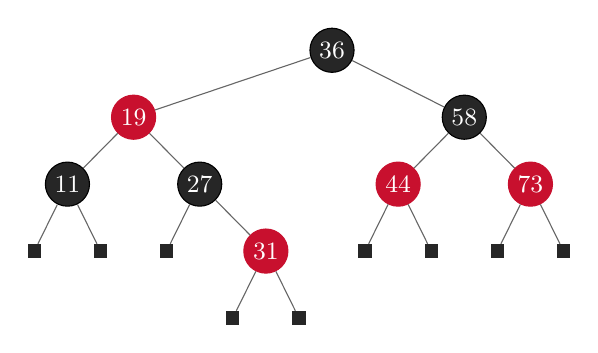
\begin{tikzpicture}[x=0.42cm,y=0.85cm,baseline=(current bounding box.north)]
\node[tnil] (rbdefNIL) at (0,-3) {};
\node[tnB] (rbdef11) at (1,-2) {11};
\node[tnil] (rbdefnil2) at (2,-3) {};
\node[tnR] (rbdef19) at (3,-1) {19};
\node[tnil] (rbdefnil4) at (4,-3) {};
\node[tnB] (rbdef27) at (5,-2) {27};
\node[tnil] (rbdefnil6) at (6,-4) {};
\node[tnR] (rbdef31) at (7,-3) {31};
\node[tnil] (rbdefnil8) at (8,-4) {};
\node[tnB] (rbdef36) at (9,0) {36};
\node[tnil] (rbdefnil10) at (10,-3) {};
\node[tnR] (rbdef44) at (11,-2) {44};
\node[tnil] (rbdefnil12) at (12,-3) {};
\node[tnB] (rbdef58) at (13,-1) {58};
\node[tnil] (rbdefnil14) at (14,-3) {};
\node[tnR] (rbdef73) at (15,-2) {73};
\node[tnil] (rbdefnil16) at (16,-3) {};
\draw[te] (rbdef36) -- (rbdef19);
\draw[te] (rbdef19) -- (rbdef11);
\draw[te] (rbdef11) -- (rbdefNIL);
\draw[te] (rbdef11) -- (rbdefnil2);
\draw[te] (rbdef19) -- (rbdef27);
\draw[te] (rbdef27) -- (rbdefnil4);
\draw[te] (rbdef27) -- (rbdef31);
\draw[te] (rbdef31) -- (rbdefnil6);
\draw[te] (rbdef31) -- (rbdefnil8);
\draw[te] (rbdef36) -- (rbdef58);
\draw[te] (rbdef58) -- (rbdef44);
\draw[te] (rbdef44) -- (rbdefnil10);
\draw[te] (rbdef44) -- (rbdefnil12);
\draw[te] (rbdef58) -- (rbdef73);
\draw[te] (rbdef73) -- (rbdefnil14);
\draw[te] (rbdef73) -- (rbdefnil16);
\end{tikzpicture}
\diagcaption{一棵紅黑樹，小方塊是 NIL。 根 $36$ 的黑高是 $2$：例如
$36 \to 19 \to 11 \to \text{NIL}$ 經過 $11$、NIL 兩個黑色；$36 \to 58 \to 44 \to
\text{NIL}$ 經過 $58$、NIL。 $19$ 和 $58$ 的黑高都是 $1$。}
\label{fig:bal-rbdef}
\end{center}

之後的圖不再畫 NIL，但要記得它們在那裡：例如 $27$ 只有一個紅色的右子節點 $31$，它
的左邊是一個 NIL，$27 \to \text{NIL}$ 和 $27 \to 31 \to \text{NIL}$ 都只有一個黑色
（NIL），所以 $27$ 是合法的。 如果 $31$ 是黑的，右邊那條就有兩個黑色，違反第 5 條。

\subsection{高度上界}

\begin{lemma}
\label{lem:bal-rb-count}
以 $x$ 為根的子樹至少有 $2^{\mathrm{bh}(x)} - 1$ 個內部節點。
\end{lemma}

\begin{proof}
對 $x$ 的高度歸納。 $x$ 是 NIL 時，$\mathrm{bh}(x) = 0$，子樹有 $0 = 2^0 - 1$ 個內部
節點。 $x$ 是內部節點時，它的子節點 $c$ 如果是紅的，$\mathrm{bh}(c) = \mathrm{bh}(x)$；
如果是黑的，$\mathrm{bh}(c) = \mathrm{bh}(x) - 1$。 不管哪種，兩個子節點的黑高都至
少 $\mathrm{bh}(x) - 1$，而且子樹比較矮，由歸納假設各至少有 $2^{\mathrm{bh}(x)-1} - 1$
個內部節點。 加上 $x$ 自己：
\[
2\bigl(2^{\mathrm{bh}(x)-1} - 1\bigr) + 1 = 2^{\mathrm{bh}(x)} - 1. \qedhere
\]
\end{proof}

\begin{theorem}
\label{thm:bal-rb-height}
有 $n$ 個內部節點的紅黑樹，高度 $h \le 2 \lg(n + 1)$。
\end{theorem}

\begin{proof}
取一條最長的路徑，從根經過 $h$ 個內部節點 $v_1 = \text{根}, v_2, \ldots, v_h$ 走到一
個 NIL。 看 $v_2, \ldots, v_h$ 加上最後的 NIL，共 $h$ 個節點。 由第 4 條，紅色節點
的下一個一定是黑色，所以每個紅色節點都可以和它下一個節點配成一對，各對互不重疊；
沒配到的都是黑色。 因此這 $h$ 個節點裡黑色至少佔一半，$\mathrm{bh}(\text{根}) \ge
h/2$。 由引理~\ref{lem:bal-rb-count}，$n \ge 2^{h/2} - 1$，移項取對數得到
$h \le 2\lg(n+1)$。
\end{proof}

證明用到的事實是：任何一條路徑上，紅色不會比黑色多。 所以同一個節點往下的最長路
徑，不會超過最短路徑的兩倍（觀念題第 9 題）。 這比 AVL 的條件寬，$2$ 對上 $1.44$，
換來的是插入、刪除時要調整的地方比較少。

搜尋和二元搜尋樹完全一樣，不看顏色，$O(\lg n)$。 要處理的是插入和刪除：照二元搜尋
樹的方法改完之後，顏色可能違反性質，要用改色和旋轉修回來。

\subsection{帶父指標的旋轉}

紅黑樹修正時要往上看父節點、祖父節點和叔叔（父節點的兄弟），所以節點多存一個父指
標 $p$，旋轉時三組父子關係都要雙向更新。 下面是左旋，右旋把 $\mathit{left}$、
$\mathit{right}$ 對調。

\begin{pseudo}[label=alg:bal-left-rotate]{帶父指標的左旋：$a$ 的右子節點 $b$ 升上來}
\Procedure{Left-Rotate}{$T, a$}
    \State $b \gets a.\mathit{right}$
    \State $a.\mathit{right} \gets b.\mathit{left}$ \Comment{$b$ 靠內側的子樹給 $a$}
    \If{$b.\mathit{left} \ne \NIL$}
        \State $b.\mathit{left}.p \gets a$
    \EndIf
    \State $b.p \gets a.p$ \Comment{$b$ 接到 $a$ 原本的位置}
    \If{$a.p = \NIL$}
        \State $T.\mathit{root} \gets b$
    \ElsIf{$a = a.p.\mathit{left}$}
        \State $a.p.\mathit{left} \gets b$
    \Else
        \State $a.p.\mathit{right} \gets b$
    \EndIf
    \State $b.\mathit{left} \gets a$
    \State $a.p \gets b$
\EndProcedure
\end{pseudo}

\subsection{插入}
\label{sec:bal-rb-insert}

先照二元搜尋樹插入新節點 $z$，\textbf{塗成紅色}。 紅色節點不改變任何路徑上的黑色個
數，所以第 5 條不會壞；第 1、3 條也不會壞。 可能壞的只有兩條：
\begin{itemize}
\item 第 2 條：$z$ 是根（原本是空樹）。 把它改成黑色就好。
\item 第 4 條：$z$ 的父節點 $p$ 也是紅的。 這時 $p$ 不是根（根是黑的），所以祖父
$g$ 存在，而且 $g$ 是黑的（樹原本合法，$p$ 紅則 $g$ 黑）。
\end{itemize}

修第 4 條時，關鍵是叔叔 $u$（$g$ 的另一個子節點）的顏色。 下面假設 $p$ 是 $g$ 的
左子節點，右邊的情況左右對調。

\begin{itemize}
\item \textbf{情況 1：$u$ 是紅的。} 把 $p$、$u$ 改黑，$g$ 改紅。 經過 $g$ 的每條路徑，
少了 $g$ 一個黑色、多了 $p$ 或 $u$ 一個黑色，個數不變。 $z$ 和 $p$ 不再紅紅相連，但
$g$ 變紅之後，它的父節點可能是紅的。 把 $z$ 移到 $g$，往上兩層繼續檢查。
\item \textbf{情況 2：$u$ 是黑的，$z$ 是 $p$ 的右子節點（內側）。} 把 $z$ 移到 $p$，
對新的 $z$ 左旋。 兩個紅色節點換了上下，紅紅相連還在，但現在是外側，變成情況 3。
這次旋轉只動兩個紅色節點，路徑上的黑色個數不變。
\item \textbf{情況 3：$u$ 是黑的，$z$ 是 $p$ 的左子節點（外側）。} $p$ 改黑，$g$ 改
紅，對 $g$ 右旋。 $p$ 升上來，黑色的 $p$ 取代了原本黑色的 $g$ 的位置，左右兩邊的黑
色個數都和原本一樣，而且 $p$ 是黑的，上面不會有紅紅相連，修正結束。
\end{itemize}

迴圈結束時（$p$ 是黑的，或 $z$ 走到了根），最後把根塗黑。 情況 1 只有在 $g$ 變紅時
才可能讓根變紅，這一步正是處理它。

\begin{center}
\begin{tikzpicture}[x=0.75cm, y=0.8cm]
% 情況 1
\node[font=\small\bfseries, anchor=west] at (-2.4,0.7) {情況 1};
\node[tnB] (g) at (0,0) {$g$};
\node[tnR] (p) at (-1.2,-1) {$p$};
\node[tnR] (u) at (1.2,-1) {$u$};
\node[tnR] (z) at (-1.8,-2) {$z$};
\draw[te] (g) -- (p); \draw[te] (g) -- (u); \draw[te] (p) -- (z); \draw[te] (p) -- (-0.6,-2.0);
\subtri[0.7]{-0.6}{-2.0}{3}
\draw[tarr] (2.0,-1) -- node[above, font=\scriptsize] {改色} (3.3,-1);
\begin{scope}[xshift=4.4cm]
\node[tnR] (g) at (0,0) {$g$};
\node[tnB] (p) at (-1.2,-1) {$p$};
\node[tnB] (u) at (1.2,-1) {$u$};
\node[tnR] (z) at (-1.8,-2) {};
\draw[te] (g) -- (p); \draw[te] (g) -- (u); \draw[te] (p) -- (z); \draw[te] (p) -- (-0.6,-2.0);
\subtri[0.7]{-0.6}{-2.0}{3}
\node[annl, anchor=south east] at (g.north west) {新的 $z$};
\end{scope}
% 情況 2 → 3
\begin{scope}[yshift=-3.6cm]
\node[font=\small\bfseries, anchor=west] at (-2.4,0.7) {情況 2};
\node[tnB] (g) at (0,0) {$g$};
\node[tnR] (p) at (-1.2,-1) {$p$};
\node[tnB] (u) at (1.2,-1) {$u$};
\node[tnR] (z) at (-0.6,-2) {$z$};
\draw[te] (g) -- (p); \draw[te] (g) -- (u); \draw[te] (p) -- (-1.8,-2.0); \draw[te] (p) -- (z);
\draw[te] (z) -- (-1.0,-3.0); \draw[te] (z) -- (-0.2,-3.0);
\subtri[0.7]{-1.8}{-2.0}{1}
\subtri[0.7]{-1.0}{-3.0}{2}
\subtri[0.7]{-0.2}{-3.0}{3}
\draw[tarr] (2.0,-1) -- node[above, font=\scriptsize] {左旋 $p$} (3.3,-1);
\begin{scope}[xshift=4.4cm]
\node[tnB] (g) at (0,0) {$g$};
\node[tnR] (z) at (-1.2,-1) {$z'$};
\node[tnB] (u) at (1.2,-1) {$u$};
\node[tnR] (p) at (-1.8,-2) {$p'$};
\draw[te] (g) -- (z); \draw[te] (g) -- (u); \draw[te] (z) -- (p); \draw[te] (z) -- (-0.6,-2.0);
\draw[te] (p) -- (-2.2,-3.0); \draw[te] (p) -- (-1.4,-3.0);
\subtri[0.7]{-2.2}{-3.0}{1}
\subtri[0.7]{-1.4}{-3.0}{2}
\subtri[0.7]{-0.6}{-2.0}{3}
\end{scope}
\end{scope}
% 情況 3
\begin{scope}[xshift=9.6cm]
\node[font=\small\bfseries, anchor=west] at (-2.4,0.7) {情況 3};
\node[tnB] (g) at (0,0) {$g$};
\node[tnR] (p) at (-1.2,-1) {$p$};
\node[tnB] (u) at (1.2,-1) {$u$};
\node[tnR] (z) at (-1.8,-2) {$z$};
\draw[te] (g) -- (p); \draw[te] (g) -- (u); \draw[te] (p) -- (z); \draw[te] (p) -- (-0.6,-2.0);
\subtri[0.7]{-0.6}{-2.0}{3}
\draw[tarr] (0,-2.9) -- node[right, font=\scriptsize] {右旋 $g$、改色} (0,-3.9);
\begin{scope}[yshift=-4.4cm]
\node[tnB] (p) at (0,0) {$p$};
\node[tnR] (z) at (-1.2,-1) {$z$};
\node[tnR] (g) at (1.2,-1) {$g$};
\node[tnB] (u) at (1.8,-2) {$u$};
\draw[te] (p) -- (z); \draw[te] (p) -- (g); \draw[te] (g) -- (0.6,-2.0); \draw[te] (g) -- (u);
\subtri[0.7]{0.6}{-2.0}{3}
\end{scope}
\end{scope}
\end{tikzpicture}
\diagcaption{插入的三種情況（$p$ 是 $g$ 的左子節點）。 三角形是黑高相同的子樹，
$z$ 本身的子樹沒有畫。 情況 1 的 $z$ 也可以是 $p$ 的右子節點，做法一樣。 情況 2
左旋之後，$z'$（原本的 $z$）和 $p'$（原本的 $p$）換了上下，再接情況 3：這時的
「$z$」是 $p'$，「$p$」是 $z'$。}
\label{fig:bal-rb-insert-cases}
\end{center}

\proc{RB-Insert}$(T, k)$ 和第~9~章的插入相同：從根往下找到位置，新節點 $z$ 的父指標
設成找到的父節點，兩個子指標是 \NIL，顏色是紅色；接好之後呼叫
\proc{RB-Insert-Fixup}$(T, z)$。

\begin{pseudo}[label=alg:bal-rb-fixup]{插入後的修正}
\Procedure{RB-Insert-Fixup}{$T, z$}
    \While{$z.p$ 是紅的}
        \State $p \gets z.p$
        \State $g \gets p.p$
        \If{$p = g.\mathit{left}$}
            \State $u \gets g.\mathit{right}$
            \If{$u$ 是紅的} \Comment{情況 1}
                \State $p$、$u$ 改黑，$g$ 改紅
                \State $z \gets g$
            \Else
                \If{$z = p.\mathit{right}$} \Comment{情況 2}
                    \State $z \gets p$
                    \State \Call{Left-Rotate}{$T, z$}
                    \State $p \gets z.p$
                \EndIf
                \State $p$ 改黑，$g$ 改紅 \Comment{情況 3}
                \State \Call{Right-Rotate}{$T, g$}
            \EndIf
        \Else
            \State 和第 6 到 16 行相同，$\mathit{left}$、$\mathit{right}$ 對調，\proc{Left-Rotate}、\proc{Right-Rotate} 對調
        \EndIf
    \EndWhile
    \State $T.\mathit{root}$ 改黑
\EndProcedure
\end{pseudo}

NIL 一律當成黑色：$z$ 是根時 $z.p = \NIL$，第 2 行的條件不成立；叔叔是 NIL 時，它
是黑的，走情況 2 或 3。

\textbf{成本。} 情況 1 讓 $z$ 往上兩層，最多做 $O(\lg n)$ 次，每次只改顏色。 情況 2
最多一次，接著情況 3 一次，做完迴圈就結束。 所以插入一共最多\textbf{兩次旋轉}，時間
$O(\lg n)$。

\subsection{插入的完整追蹤}
\label{sec:bal-rb-trace}

依序插入
\[
85,\ 28,\ 24,\ 87,\ 75,\ 50,\ 69,\ 46,\ 52,\ 35 .
\]
圖上深色是黑節點，紅底是紅節點，「$z$」標的是目前要檢查的節點。 每一步的說明寫
在圖下；「情況 3」之類的字，指的是\textbf{接下來}要做的事。

\begin{center}
\begin{tikzpicture}[x=0.5cm,y=0.7cm,baseline=(current bounding box.north)]
\node[tnB] (ria85) at (0,0) {85};
\node[plab] at (0.0,-2.75) {(a) 插入 85，根改黑};
\end{tikzpicture}\hspace{0.5cm}\begin{tikzpicture}[x=0.5cm,y=0.7cm,baseline=(current bounding box.north)]
\node[tnR] (rib24) at (0,-2) {24};
\node[tnR] (rib28) at (1,-1) {28};
\node[tnB] (rib85) at (2,0) {85};
\draw[te] (rib85) -- (rib28);
\draw[te] (rib28) -- (rib24);
\node[annl, anchor=south east] at (rib24.north west) {$z$};
\node[plab] at (1.0,-2.75) {(b) 插入 28、24：情況 3};
\end{tikzpicture}\hspace{0.5cm}\begin{tikzpicture}[x=0.5cm,y=0.7cm,baseline=(current bounding box.north)]
\node[tnR] (ric24) at (0,-1) {24};
\node[tnB] (ric28) at (1,0) {28};
\node[tnR] (ric85) at (2,-1) {85};
\draw[te] (ric28) -- (ric24);
\draw[te] (ric28) -- (ric85);
\node[plab] at (1.0,-2.75) {(c) 右旋 85 之後};
\end{tikzpicture}\\*[0.6em]
\begin{tikzpicture}[x=0.5cm,y=0.7cm,baseline=(current bounding box.north)]
\node[tnR] (rid24) at (0,-1) {24};
\node[tnB] (rid28) at (1,0) {28};
\node[tnR] (rid85) at (2,-1) {85};
\node[tnR] (rid87) at (3,-2) {87};
\draw[te] (rid28) -- (rid24);
\draw[te] (rid28) -- (rid85);
\draw[te] (rid85) -- (rid87);
\node[annl, anchor=south east] at (rid87.north west) {$z$};
\node[plab] at (1.5,-2.75) {(d) 插入 87：情況 1};
\end{tikzpicture}\hspace{0.6cm}\begin{tikzpicture}[x=0.5cm,y=0.7cm,baseline=(current bounding box.north)]
\node[tnB] (rie24) at (0,-1) {24};
\node[tnB] (rie28) at (1,0) {28};
\node[tnB] (rie85) at (2,-1) {85};
\node[tnR] (rie87) at (3,-2) {87};
\draw[te] (rie28) -- (rie24);
\draw[te] (rie28) -- (rie85);
\draw[te] (rie85) -- (rie87);
\node[plab] at (1.5,-2.75) {(e) 改色、根改回黑};
\end{tikzpicture}
\diagcaption{插入 $85$ 到 $87$。}
\label{fig:bal-rb-trace1}
\end{center}

\begin{itemize}
\item $85$：樹是空的，$z$ 是根，改黑。 $28$：父節點 $85$ 是黑的，不用修。
\item $24$：父 $28$ 紅，叔叔是 $85$ 的右邊，NIL，黑的。 $24$ 是 $28$ 的左子節點、
$28$ 是 $85$ 的左子節點，在外側，情況 3：$28$ 改黑、$85$ 改紅，右旋 $85$。
\item $87$：父 $85$ 紅，叔叔 $24$ 也紅，情況 1：$85$、$24$ 改黑，$28$ 改紅。 $z$ 移到
$28$，它是根，迴圈結束，根改回黑。 這是黑高增加的唯一方式：情況 1 一路改色到根，根
被改紅再改黑，整棵樹的每條路徑同時多一個黑色。
\end{itemize}

\begin{center}
\begin{tikzpicture}[x=0.5cm,y=0.7cm,baseline=(current bounding box.north)]
\node[tnB] (rif24) at (0,-1) {24};
\node[tnB] (rif28) at (1,0) {28};
\node[tnR] (rif50) at (2,-3) {50};
\node[tnR] (rif75) at (3,-2) {75};
\node[tnB] (rif85) at (4,-1) {85};
\node[tnR] (rif87) at (5,-2) {87};
\draw[te] (rif28) -- (rif24);
\draw[te] (rif28) -- (rif85);
\draw[te] (rif85) -- (rif75);
\draw[te] (rif75) -- (rif50);
\draw[te] (rif85) -- (rif87);
\node[annl, anchor=south east] at (rif50.north west) {$z$};
\node[plab] at (2.5,-4.75) {(f) 插入 75、50：情況 1};
\end{tikzpicture}\hspace{0.4cm}\begin{tikzpicture}[x=0.5cm,y=0.7cm,baseline=(current bounding box.north)]
\node[tnB] (rig24) at (0,-1) {24};
\node[tnB] (rig28) at (1,0) {28};
\node[tnR] (rig50) at (2,-3) {50};
\node[tnB] (rig75) at (3,-2) {75};
\node[tnR] (rig85) at (4,-1) {85};
\node[tnB] (rig87) at (5,-2) {87};
\draw[te] (rig28) -- (rig24);
\draw[te] (rig28) -- (rig85);
\draw[te] (rig85) -- (rig75);
\draw[te] (rig75) -- (rig50);
\draw[te] (rig85) -- (rig87);
\node[plab] at (2.5,-4.75) {(g) 改色之後};
\end{tikzpicture}\hspace{0.4cm}\begin{tikzpicture}[x=0.5cm,y=0.7cm,baseline=(current bounding box.north)]
\node[tnB] (rih24) at (0,-1) {24};
\node[tnB] (rih28) at (1,0) {28};
\node[tnR] (rih50) at (2,-3) {50};
\node[tnR] (rih69) at (3,-4) {69};
\node[tnB] (rih75) at (4,-2) {75};
\node[tnR] (rih85) at (5,-1) {85};
\node[tnB] (rih87) at (6,-2) {87};
\draw[te] (rih28) -- (rih24);
\draw[te] (rih28) -- (rih85);
\draw[te] (rih85) -- (rih75);
\draw[te] (rih75) -- (rih50);
\draw[te] (rih50) -- (rih69);
\draw[te] (rih85) -- (rih87);
\node[annl, anchor=south east] at (rih69.north west) {$z$};
\node[plab] at (3.0,-4.75) {(h) 插入 69：情況 2};
\end{tikzpicture}\\*[0.6em]
\begin{tikzpicture}[x=0.5cm,y=0.7cm,baseline=(current bounding box.north)]
\node[tnB] (rii24) at (0,-1) {24};
\node[tnB] (rii28) at (1,0) {28};
\node[tnR] (rii50) at (2,-4) {50};
\node[tnR] (rii69) at (3,-3) {69};
\node[tnB] (rii75) at (4,-2) {75};
\node[tnR] (rii85) at (5,-1) {85};
\node[tnB] (rii87) at (6,-2) {87};
\draw[te] (rii28) -- (rii24);
\draw[te] (rii28) -- (rii85);
\draw[te] (rii85) -- (rii75);
\draw[te] (rii75) -- (rii69);
\draw[te] (rii69) -- (rii50);
\draw[te] (rii85) -- (rii87);
\node[annl, anchor=south east] at (rii50.north west) {$z$};
\node[plab] at (3.0,-4.75) {(i) 左旋 50：情況 3};
\end{tikzpicture}\hspace{0.4cm}\begin{tikzpicture}[x=0.5cm,y=0.7cm,baseline=(current bounding box.north)]
\node[tnB] (rij24) at (0,-1) {24};
\node[tnB] (rij28) at (1,0) {28};
\node[tnR] (rij50) at (2,-3) {50};
\node[tnB] (rij69) at (3,-2) {69};
\node[tnR] (rij75) at (4,-3) {75};
\node[tnR] (rij85) at (5,-1) {85};
\node[tnB] (rij87) at (6,-2) {87};
\draw[te] (rij28) -- (rij24);
\draw[te] (rij28) -- (rij85);
\draw[te] (rij85) -- (rij69);
\draw[te] (rij69) -- (rij50);
\draw[te] (rij69) -- (rij75);
\draw[te] (rij85) -- (rij87);
\node[plab] at (3.0,-4.75) {(j) 右旋 75 之後};
\end{tikzpicture}
\diagcaption{插入 $75$、$50$、$69$。}
\label{fig:bal-rb-trace2}
\end{center}

\begin{itemize}
\item $75$：父 $85$ 黑，不用修。
\item $50$：父 $75$ 紅，叔叔 $87$ 紅，情況 1：$75$、$87$ 改黑，$85$ 改紅。 $z$ 移到
$85$，它的父節點 $28$ 是黑的，結束。
\item $69$：父 $50$ 紅；$50$ 是 $75$ 的左子節點，叔叔是 $75$ 的右邊（NIL），黑的。
$69$ 是 $50$ 的右子節點，在內側，情況 2：$z$ 移到 $50$，左旋 $50$，$69$ 升上來，
(i)。 現在 $z = 50$ 是 $69$ 的左子節點，在外側，情況 3：$69$ 改黑、$75$ 改紅，右
旋 $75$，(j)。
\end{itemize}

\begin{center}
\begin{tikzpicture}[x=0.5cm,y=0.7cm,baseline=(current bounding box.north)]
\node[tnB] (rik24) at (0,-1) {24};
\node[tnB] (rik28) at (1,0) {28};
\node[tnR] (rik46) at (2,-4) {46};
\node[tnR] (rik50) at (3,-3) {50};
\node[tnB] (rik69) at (4,-2) {69};
\node[tnR] (rik75) at (5,-3) {75};
\node[tnR] (rik85) at (6,-1) {85};
\node[tnB] (rik87) at (7,-2) {87};
\draw[te] (rik28) -- (rik24);
\draw[te] (rik28) -- (rik85);
\draw[te] (rik85) -- (rik69);
\draw[te] (rik69) -- (rik50);
\draw[te] (rik50) -- (rik46);
\draw[te] (rik69) -- (rik75);
\draw[te] (rik85) -- (rik87);
\node[annl, anchor=south east] at (rik46.north west) {$z$};
\node[plab] at (3.5,-4.75) {(k) 插入 46：情況 1};
\end{tikzpicture}\hspace{0.4cm}\begin{tikzpicture}[x=0.5cm,y=0.7cm,baseline=(current bounding box.north)]
\node[tnB] (ril24) at (0,-1) {24};
\node[tnB] (ril28) at (1,0) {28};
\node[tnR] (ril46) at (2,-4) {46};
\node[tnB] (ril50) at (3,-3) {50};
\node[tnR] (ril69) at (4,-2) {69};
\node[tnB] (ril75) at (5,-3) {75};
\node[tnR] (ril85) at (6,-1) {85};
\node[tnB] (ril87) at (7,-2) {87};
\draw[te] (ril28) -- (ril24);
\draw[te] (ril28) -- (ril85);
\draw[te] (ril85) -- (ril69);
\draw[te] (ril69) -- (ril50);
\draw[te] (ril50) -- (ril46);
\draw[te] (ril69) -- (ril75);
\draw[te] (ril85) -- (ril87);
\node[annl, anchor=south east] at (ril69.north west) {$z$};
\node[plab] at (3.5,-4.75) {(l) 改色後 $z = 69$：情況 2};
\end{tikzpicture}\\*[0.6em]
\begin{tikzpicture}[x=0.5cm,y=0.7cm,baseline=(current bounding box.north)]
\node[tnB] (rim24) at (0,-1) {24};
\node[tnB] (rim28) at (1,0) {28};
\node[tnR] (rim46) at (2,-3) {46};
\node[tnB] (rim50) at (3,-2) {50};
\node[tnR] (rim69) at (4,-1) {69};
\node[tnB] (rim75) at (5,-3) {75};
\node[tnR] (rim85) at (6,-2) {85};
\node[tnB] (rim87) at (7,-3) {87};
\draw[te] (rim28) -- (rim24);
\draw[te] (rim28) -- (rim69);
\draw[te] (rim69) -- (rim50);
\draw[te] (rim50) -- (rim46);
\draw[te] (rim69) -- (rim85);
\draw[te] (rim85) -- (rim75);
\draw[te] (rim85) -- (rim87);
\node[annl, anchor=south east] at (rim85.north west) {$z$};
\node[plab] at (3.5,-4.75) {(m) 右旋 85：情況 3};
\end{tikzpicture}\hspace{0.4cm}\begin{tikzpicture}[x=0.5cm,y=0.7cm,baseline=(current bounding box.north)]
\node[tnB] (rin24) at (0,-2) {24};
\node[tnR] (rin28) at (1,-1) {28};
\node[tnR] (rin46) at (2,-3) {46};
\node[tnB] (rin50) at (3,-2) {50};
\node[tnB] (rin69) at (4,0) {69};
\node[tnB] (rin75) at (5,-2) {75};
\node[tnR] (rin85) at (6,-1) {85};
\node[tnB] (rin87) at (7,-2) {87};
\draw[te] (rin69) -- (rin28);
\draw[te] (rin28) -- (rin24);
\draw[te] (rin28) -- (rin50);
\draw[te] (rin50) -- (rin46);
\draw[te] (rin69) -- (rin85);
\draw[te] (rin85) -- (rin75);
\draw[te] (rin85) -- (rin87);
\node[plab] at (3.5,-4.75) {(n) 左旋 28 之後};
\end{tikzpicture}
\diagcaption{插入 $46$：情況 1 之後接著情況 2、情況 3。}
\label{fig:bal-rb-trace3}
\end{center}

\begin{itemize}
\item $46$：父 $50$ 紅，叔叔 $75$ 紅，情況 1：$50$、$75$ 改黑，$69$ 改紅，$z$ 移到
$69$，(l)。 $69$ 的父節點 $85$ 是紅的，還要修。 這次 $p = 85$ 是祖父 $28$ 的
\textbf{右}子節點，用左右對調的版本：叔叔是 $24$，黑的；$z = 69$ 是 $85$ 的左子節
點，在內側，情況 2：$z$ 移到 $85$，右旋 $85$，(m)。 接著情況 3：$69$ 改黑、$28$
改紅，左旋 $28$，$69$ 成為新的根，(n)。
\end{itemize}

\begin{center}
\begin{tikzpicture}[x=0.5cm,y=0.7cm,baseline=(current bounding box.north)]
\node[tnB] (rio24) at (0,-2) {24};
\node[tnR] (rio28) at (1,-1) {28};
\node[tnR] (rio35) at (2,-4) {35};
\node[tnR] (rio46) at (3,-3) {46};
\node[tnB] (rio50) at (4,-2) {50};
\node[tnR] (rio52) at (5,-3) {52};
\node[tnB] (rio69) at (6,0) {69};
\node[tnB] (rio75) at (7,-2) {75};
\node[tnR] (rio85) at (8,-1) {85};
\node[tnB] (rio87) at (9,-2) {87};
\draw[te] (rio69) -- (rio28);
\draw[te] (rio28) -- (rio24);
\draw[te] (rio28) -- (rio50);
\draw[te] (rio50) -- (rio46);
\draw[te] (rio46) -- (rio35);
\draw[te] (rio50) -- (rio52);
\draw[te] (rio69) -- (rio85);
\draw[te] (rio85) -- (rio75);
\draw[te] (rio85) -- (rio87);
\node[annl, anchor=south east] at (rio35.north west) {$z$};
\node[plab] at (4.5,-4.75) {(o) 插入 52、35：情況 1};
\end{tikzpicture}\hspace{0.5cm}\begin{tikzpicture}[x=0.5cm,y=0.7cm,baseline=(current bounding box.north)]
\node[tnB] (rip24) at (0,-2) {24};
\node[tnR] (rip28) at (1,-1) {28};
\node[tnR] (rip35) at (2,-4) {35};
\node[tnB] (rip46) at (3,-3) {46};
\node[tnR] (rip50) at (4,-2) {50};
\node[tnB] (rip52) at (5,-3) {52};
\node[tnB] (rip69) at (6,0) {69};
\node[tnB] (rip75) at (7,-2) {75};
\node[tnR] (rip85) at (8,-1) {85};
\node[tnB] (rip87) at (9,-2) {87};
\draw[te] (rip69) -- (rip28);
\draw[te] (rip28) -- (rip24);
\draw[te] (rip28) -- (rip50);
\draw[te] (rip50) -- (rip46);
\draw[te] (rip46) -- (rip35);
\draw[te] (rip50) -- (rip52);
\draw[te] (rip69) -- (rip85);
\draw[te] (rip85) -- (rip75);
\draw[te] (rip85) -- (rip87);
\node[annl, anchor=south east] at (rip50.north west) {$z$};
\node[plab] at (4.5,-4.75) {(p) 改色後 $z = 50$：情況 1};
\end{tikzpicture}\\*[0.6em]
\begin{tikzpicture}[x=0.5cm,y=0.7cm,baseline=(current bounding box.north)]
\node[tnB] (riq24) at (0,-2) {24};
\node[tnB] (riq28) at (1,-1) {28};
\node[tnR] (riq35) at (2,-4) {35};
\node[tnB] (riq46) at (3,-3) {46};
\node[tnR] (riq50) at (4,-2) {50};
\node[tnB] (riq52) at (5,-3) {52};
\node[tnB] (riq69) at (6,0) {69};
\node[tnB] (riq75) at (7,-2) {75};
\node[tnB] (riq85) at (8,-1) {85};
\node[tnB] (riq87) at (9,-2) {87};
\draw[te] (riq69) -- (riq28);
\draw[te] (riq28) -- (riq24);
\draw[te] (riq28) -- (riq50);
\draw[te] (riq50) -- (riq46);
\draw[te] (riq46) -- (riq35);
\draw[te] (riq50) -- (riq52);
\draw[te] (riq69) -- (riq85);
\draw[te] (riq85) -- (riq75);
\draw[te] (riq85) -- (riq87);
\node[plab] at (4.5,-4.75) {(q) 改色、根改回黑};
\end{tikzpicture}
\diagcaption{插入 $52$、$35$：情況 1 連續兩次，改色一路到根。}
\label{fig:bal-rb-trace4}
\end{center}

\begin{itemize}
\item $52$：父 $50$ 黑，不用修。
\item $35$：父 $46$ 紅，叔叔 $52$ 紅，情況 1：$46$、$52$ 改黑，$50$ 改紅，$z$ 移到
$50$，(p)。 $50$ 的父節點 $28$ 紅，叔叔 $85$ 也紅，再一次情況 1：$28$、$85$ 改黑，
$69$ 改紅，$z$ 移到根 $69$。 最後根改回黑，(q)。
\end{itemize}

\begin{center}
\begin{tabular}{cll}
\toprule
插入 & 情況（L／R：父節點是祖父的左／右子節點） & 旋轉次數 \\
\midrule
85 & 根改黑 & 0 \\
28、75、52 & 不用修 & 0 \\
24 & 3L & 1 \\
87 & 1R，根改黑 & 0 \\
50 & 1L & 0 \\
69 & 2L、3L & 2 \\
46 & 1L、2R、3R & 2 \\
35 & 1L、1L，根改黑 & 0 \\
\bottomrule
\end{tabular}
\end{center}

最後的樹黑高是 $3$，高度 $5$。 同樣十個鍵放進 AVL 樹，高度是 $4$；紅黑樹允許比較
不整齊的形狀。

\begin{examnote}
紅黑樹的追蹤題，每一步先寫出 $z$、父節點、叔叔的顏色和用了哪個情況，再畫樹；情況
1 之後 $z$ 往上移了兩層，要用新的 $z$ 重新判斷。 考卷通常只能用一種顏色的筆，紅色
節點畫成雙圈或在旁邊標 R，並在答案開頭說明記號。
\end{examnote}

\subsection{C 程式}
\label{sec:bal-rb-c}

C 程式用 \texttt{NULL} 當 NIL，\texttt{is\_red} 把 \texttt{NULL} 當成黑色，這樣叔叔
是 NIL 的情況不用另外寫。 \texttt{replace\_child} 處理「把 $x$ 原本的位置交給另一個
節點」，左旋和右旋都用它。 \texttt{black\_count} 從下往上檢查第 4、5 條，順便算出
黑高。

\begin{example}[label=ex:bal-rb-insert]{c}{(rb\_insert.c) 紅黑樹的插入}
#include <stdio.h>
#include <stdlib.h>

typedef enum { RED, BLACK } Color;

typedef struct RBNode {
    int key;
    Color color;
    struct RBNode *left, *right, *parent;
} RBNode;

typedef struct {
    RBNode *root;
} RBTree;

// NULL 當成 NIL 葉子，NIL 是黑的。
static int is_red(const RBNode *x)
{
    return x != NULL && x->color == RED;
}

// 把 child 接到 x 原本在父節點底下的位置（x 是根時改 t->root）。
static void replace_child(RBTree *t, RBNode *x, RBNode *child)
{
    child->parent = x->parent;
    if (x->parent == NULL) {
        t->root = child;
    } else if (x == x->parent->left) {
        x->parent->left = child;
    } else {
        x->parent->right = child;
    }
}

static void rotate_left(RBTree *t, RBNode *x)   // x 的右子節點 y 轉上來
{
    RBNode *y = x->right;
    x->right = y->left;
    if (y->left != NULL) {
        y->left->parent = x;
    }
    replace_child(t, x, y);
    y->left = x;
    x->parent = y;
}

static void rotate_right(RBTree *t, RBNode *x)  // x 的左子節點 y 轉上來
{
    RBNode *y = x->left;
    x->left = y->right;
    if (y->right != NULL) {
        y->right->parent = x;
    }
    replace_child(t, x, y);
    y->right = x;
    x->parent = y;
}

static int reported = 0;        // 這次插入印了幾項

static void report(const char *what, char side)
{
    reported++;
    printf(" %s", what);
    if (side != '\0') {
        putchar(side);
    }
}

// 修正紅紅相連。印出用到的情況：1、2、3 後面的 L／R 表示父節點是祖父的
// 左／右子節點。
static void insert_fixup(RBTree *t, RBNode *z)
{
    while (is_red(z->parent)) {
        RBNode *p = z->parent, *g = p->parent;  // p 是紅的，所以不是根，g 存在
        int left = (p == g->left);
        RBNode *u = left ? g->right : g->left;  // 叔叔
        char side = left ? 'L' : 'R';
        if (is_red(u)) {                        // 情況 1：叔叔是紅的，改色
            report("1", side);
            p->color = BLACK;
            u->color = BLACK;
            g->color = RED;
            z = g;
            continue;
        }
        if (left && z == p->right) {            // 情況 2：z 在內側，先轉成外側
            report("2", side);
            z = p;
            rotate_left(t, z);
        } else if (!left && z == p->left) {
            report("2", side);
            z = p;
            rotate_right(t, z);
        }
        report("3", side);                      // 情況 3：z 在外側
        z->parent->color = BLACK;
        g->color = RED;
        if (left) {
            rotate_right(t, g);
        } else {
            rotate_left(t, g);
        }
    }
    if (t->root->color == RED) {
        report("root", '\0');
        t->root->color = BLACK;
    }
}

// 插入 key；key 已經在樹裡就不插。
void rb_insert(RBTree *t, int key)
{
    RBNode *y = NULL, *x = t->root;
    while (x != NULL) {                         // 和二元搜尋樹一樣找位置
        y = x;
        if (key == x->key) {
            return;
        }
        x = key < x->key ? x->left : x->right;
    }
    RBNode *z = malloc(sizeof *z);
    if (z == NULL) {
        exit(1);
    }
    z->key = key;
    z->color = RED;                             // 新節點一律是紅的
    z->left = z->right = NULL;
    z->parent = y;
    if (y == NULL) {
        t->root = z;
    } else if (key < y->key) {
        y->left = z;
    } else {
        y->right = z;
    }
    insert_fixup(t, z);
}

// 從 x 往下走到 NIL，路上的黑色節點數（含 x 和 NIL）。
// 有紅紅相連，或左右兩邊數出來不一樣時，回傳 -1。
static int black_count(const RBNode *x)
{
    if (x == NULL) {
        return 1;                               // NIL 是黑的
    }
    if (is_red(x) && (is_red(x->left) || is_red(x->right))) {
        return -1;
    }
    int a = black_count(x->left), b = black_count(x->right);
    if (a < 0 || a != b) {
        return -1;
    }
    return a + (x->color == BLACK);
}

void print_tree(const RBNode *x)
{
    if (x == NULL) {
        putchar('.');
        return;
    }
    printf("%d%c", x->key, x->color == RED ? 'R' : 'B');
    if (x->left != NULL || x->right != NULL) {
        putchar('(');
        print_tree(x->left);
        putchar(',');
        print_tree(x->right);
        putchar(')');
    }
}

void free_tree(RBNode *x)
{
    if (x != NULL) {
        free_tree(x->left);
        free_tree(x->right);
        free(x);
    }
}

int main(void)
{
    int keys[] = {85, 28, 24, 87, 75, 50, 69, 46, 52, 35};
    int n = sizeof keys / sizeof keys[0];
    RBTree t = {NULL};
    for (int i = 0; i < n; i++) {
        printf("insert %d:", keys[i]);
        reported = 0;
        rb_insert(&t, keys[i]);
        if (reported == 0) {
            printf(" -");
        }
        putchar('\n');
    }
    print_tree(t.root);
    putchar('\n');
    printf("black-height = %d\n", black_count(t.root) - 1);
    free_tree(t.root);
    return 0;
}
\end{example}
\iosample{}{insert 85: root \\ insert 28: - \\ insert 24: 3L \\ insert 87: 1R root \\ insert 75: - \\ insert 50: 1L \\ insert 69: 2L 3L \\ insert 46: 1L 2R 3R \\ insert 52: - \\ insert 35: 1L 1L root \\ 69B(28B(24B,50R(46B(35R,.),52B)),85B(75B,87B)) \\ black-height = 3}

輸出和上面的追蹤一致。 把 \texttt{main} 改成依序插入 $1, 2, \ldots, 10^6$，再算樹高，紅黑樹的高度
是 $37$，比 AVL 樹的 $20$（範例~\ref{ex:bal-avl-insert}）高，但仍然在定
理~\ref{thm:bal-rb-height} 的 $2 \lg(10^6+1) \approx 39.9$ 之內。

\subsection{刪除}
\label{sec:bal-rb-delete}

刪除比插入多幾種情況，但想法一樣：先照二元搜尋樹刪，再看壞了哪一條性質。

\textbf{第一步：決定真正拿掉的節點。} 要刪的節點 $z$ 有兩個子節點時，把後繼 $y$
（右子樹最小的節點）的鍵複製到 $z$，改成拿掉 $y$。 $y$ 沒有左子節點，所以真正被拿
掉的節點最多只有一個不是 NIL 的子節點。 下面說的「被拿掉的節點」都是指這一個，它
的顏色才是要看的顏色；$z$ 留在原位，顏色不變。 被拿掉的節點的子節點（可能是 NIL）
叫 $x$，$x$ 接到它原本的位置；$x$ 新的父節點叫 $p$。

\textbf{第二步：看被拿掉的節點的顏色。}
\begin{itemize}
\item 它是紅的：什麼都不用做。 拿掉紅色節點不改變黑色個數，它的父節點和 $x$ 都是
黑的，接起來也不會紅紅相連。
\item 它是黑的、$x$ 是紅的：把 $x$ 改黑，補回少掉的那個黑色，結束。
\item 它是黑的、$x$ 也是黑的（包括 $x$ 是 NIL）：經過 $x$ 的路徑都少了一個黑色，違
反第 5 條。 這是要修正的情況。
\end{itemize}

修正時，想像 $x$ 身上多背了一個黑色（叫它\textbf{雙重黑}），只要能把這個多出來的黑
色放到某個紅色節點上（紅改黑），或是一路推到根（直接丟掉，所有路徑一起少一個），就
修好了。 設 $x$ 是 $p$ 的左子節點，$s$ 是 $x$ 的兄弟（$p$ 的右子節點）。 $s$ 不會是
NIL：經過 $s$ 的路徑比經過 $x$ 的多一個黑色，至少有兩個黑色，所以 $s$ 是內部節點。
$s$ 靠近 $x$ 的子節點叫 $n$（$s$ 的左子節點），遠的叫 $f$（$s$ 的右子節點）。

\begin{itemize}
\item \textbf{情況 1：$s$ 是紅的。} 這時 $p$、$n$、$f$ 都是黑的。 $s$ 改黑、$p$ 改
紅，對 $p$ 左旋。 黑色個數不變，$x$ 的新兄弟是原本的 $n$，黑的，變成情況 2、3、4
之一。
\item \textbf{情況 2：$s$ 是黑的，$n$、$f$ 都是黑的。} $s$ 改紅，經過 $s$ 的路徑也少
一個黑色，和 $x$ 這邊扯平，但整棵 $p$ 的子樹少了一個黑色。 把雙重黑交給 $p$：$x$
移到 $p$。 如果 $p$ 是紅的（例如剛做完情況 1），迴圈結束，最後把它改黑就補回來
了；如果 $p$ 是黑的，往上繼續。
\item \textbf{情況 3：$s$ 是黑的，$n$ 是紅的，$f$ 是黑的。} $n$ 改黑、$s$ 改紅，對
$s$ 右旋。 $n$ 升上來當 $x$ 的新兄弟，它的遠側子節點是紅的 $s$，變成情況 4。
\item \textbf{情況 4：$s$ 是黑的，$f$ 是紅的。} $s$ 改成 $p$ 的顏色，$p$ 改黑，$f$
改黑，對 $p$ 左旋。 $x$ 這邊多了一個黑色的 $p$，抵掉雙重黑；$s$ 那邊少了 $s$ 這個
黑色，由 $f$ 改黑補回來；最上面的節點 $s$ 用的是原本 $p$ 的顏色，對更上面沒有影
響。 修正結束。
\end{itemize}

$x$ 是右子節點時，以上全部左右對調。

\begin{center}
\begin{tikzpicture}[x=0.64cm, y=0.78cm]
% 情況 1
\node[font=\small\bfseries, anchor=west] at (-2.2,0.7) {情況 1};
\node[tnB] (p) at (0,0) {$p$};
\node[tnB] (x) at (-1.2,-1) {$x$};
\node[tnR] (s) at (1.2,-1) {$s$};
\node[tnB] (n) at (0.6,-2) {$n$};
\node[tnB] (f) at (1.8,-2) {$f$};
\draw[te] (p) -- (x); \draw[te] (p) -- (s); \draw[te] (s) -- (n); \draw[te] (s) -- (f);
\draw[tarr] (2.6,-1) -- node[above, font=\scriptsize] {左旋 $p$} (4.0,-1);
\begin{scope}[xshift=5.6cm]
\node[tnB] (s) at (0,0) {$s$};
\node[tnR] (p) at (-1.2,-1) {$p$};
\node[tnB] (f) at (1.2,-1) {$f$};
\node[tnB] (x) at (-1.8,-2) {$x$};
\node[tnB] (n) at (-0.6,-2) {$n$};
\draw[te] (s) -- (p); \draw[te] (s) -- (f); \draw[te] (p) -- (x); \draw[te] (p) -- (n);
\node[annl, anchor=north] at (n.south) {新的 $s$};
\end{scope}
% 情況 2
\begin{scope}[xshift=8.3cm]
\node[font=\small\bfseries, anchor=west] at (-2.2,0.7) {情況 2};
\node[tnG] (p) at (0,0) {$p$};
\node[tnB] (x) at (-1.2,-1) {$x$};
\node[tnB] (s) at (1.2,-1) {$s$};
\node[tnB] (n) at (0.6,-2) {$n$};
\node[tnB] (f) at (1.8,-2) {$f$};
\draw[te] (p) -- (x); \draw[te] (p) -- (s); \draw[te] (s) -- (n); \draw[te] (s) -- (f);
\draw[tarr] (2.6,-1) -- node[above, font=\scriptsize] {改色} (4.0,-1);
\begin{scope}[xshift=4.0cm]
\node[tnG] (p) at (0,0) {$p$};
\node[tnB] (x) at (-1.2,-1) {};
\node[tnR] (s) at (1.2,-1) {$s$};
\node[tnB] (n) at (0.6,-2) {$n$};
\node[tnB] (f) at (1.8,-2) {$f$};
\draw[te] (p) -- (x); \draw[te] (p) -- (s); \draw[te] (s) -- (n); \draw[te] (s) -- (f);
\node[annl, anchor=south east] at (p.north west) {新的 $x$};
\end{scope}
\end{scope}
% 情況 3
\begin{scope}[yshift=-3.6cm]
\node[font=\small\bfseries, anchor=west] at (-2.2,0.7) {情況 3};
\node[tnG] (p) at (0,0) {$p$};
\node[tnB] (x) at (-1.2,-1) {$x$};
\node[tnB] (s) at (1.2,-1) {$s$};
\node[tnR] (n) at (0.6,-2) {$n$};
\node[tnB] (f) at (1.8,-2) {$f$};
\draw[te] (p) -- (x); \draw[te] (p) -- (s); \draw[te] (s) -- (n); \draw[te] (s) -- (f);
\draw[tarr] (2.6,-1) -- node[above, font=\scriptsize] {右旋 $s$} (4.0,-1);
\begin{scope}[xshift=5.0cm]
\node[tnG] (p) at (0,0) {$p$};
\node[tnB] (x) at (-1.2,-1) {$x$};
\node[tnB] (n) at (1.2,-1) {$n$};
\node[tnR] (s) at (1.8,-2) {$s$};
\node[tnB] (f) at (2.4,-3) {$f$};
\draw[te] (p) -- (x); \draw[te] (p) -- (n); \draw[te] (n) -- (s); \draw[te] (s) -- (f);
\node[annl, anchor=south west] at (n.north east) {新的 $s$};
\end{scope}
\end{scope}
% 情況 4
\begin{scope}[xshift=8.3cm, yshift=-3.6cm]
\node[font=\small\bfseries, anchor=west] at (-2.2,0.7) {情況 4};
\node[tnG] (p) at (0,0) {$p$};
\node[tnB] (x) at (-1.2,-1) {$x$};
\node[tnB] (s) at (1.2,-1) {$s$};
\node[tnG] (n) at (0.6,-2) {$n$};
\node[tnR] (f) at (1.8,-2) {$f$};
\draw[te] (p) -- (x); \draw[te] (p) -- (s); \draw[te] (s) -- (n); \draw[te] (s) -- (f);
\draw[tarr] (2.6,-1) -- node[above, font=\scriptsize] {左旋 $p$} (4.0,-1);
\begin{scope}[xshift=5.6cm]
\node[tnG] (s) at (0,0) {$s$};
\node[tnB] (p) at (-1.2,-1) {$p$};
\node[tnB] (f) at (1.2,-1) {$f$};
\node[tnB] (x) at (-1.8,-2) {$x$};
\node[tnG] (n) at (-0.6,-2) {$n$};
\draw[te] (s) -- (p); \draw[te] (s) -- (f); \draw[te] (p) -- (x); \draw[te] (p) -- (n);
\end{scope}
\end{scope}
\end{tikzpicture}
\diagcaption{刪除修正的四種情況（$x$ 是 $p$ 的左子節點）。 $x$ 是雙重黑；灰色表示
紅黑都可以，情況 4 右邊的 $s$ 用的是左邊 $p$ 的顏色。 $n$、$f$ 底下的子樹和 $x$ 的
子樹都沒有畫，它們跟著原本的父節點走，$n$ 的子樹在情況 3 會分給 $s$ 和 $n$，照
旋轉的規則（圖~\ref{fig:bal-rotation}）接。}
\label{fig:bal-rb-delete-cases}
\end{center}

\begin{pseudo}[label=alg:bal-rb-delete]{紅黑樹的刪除}
\Procedure{RB-Delete}{$T, z$}
    \If{$z.\mathit{left} \ne \NIL$ \AND $z.\mathit{right} \ne \NIL$}
        \State $y \gets z.\mathit{right}$ 一路往左走到底的節點
        \State $z.\mathit{key} \gets y.\mathit{key}$
        \State $z \gets y$ \Comment{改成拿掉後繼}
    \EndIf
    \State $x \gets z$ 不是 \NIL 的那個子節點（兩個都是 \NIL 時 $x = \NIL$）
    \State $p \gets z.p$
    \State 把 $x$ 接到 $z$ 原本的位置（$x \ne \NIL$ 時設 $x.p \gets p$；$p = \NIL$ 時 $T.\mathit{root} \gets x$）
    \If{$z$ 是黑的}
        \State \Call{RB-Delete-Fixup}{$T, x, p$}
    \EndIf
    \State 釋放 $z$
\EndProcedure
\end{pseudo}

\begin{pseudo}[label=alg:bal-rb-delfix]{刪除後的修正，$x$ 可能是 \NIL，所以另外傳父節點 $p$}
\Procedure{RB-Delete-Fixup}{$T, x, p$}
    \While{$x \ne T.\mathit{root}$ \AND $x$ 是黑的}
        \If{$x = p.\mathit{left}$}
            \State $s \gets p.\mathit{right}$
            \If{$s$ 是紅的} \Comment{情況 1}
                \State $s$ 改黑，$p$ 改紅
                \State \Call{Left-Rotate}{$T, p$}
                \State $s \gets p.\mathit{right}$
            \EndIf
            \If{$s.\mathit{left}$、$s.\mathit{right}$ 都是黑的} \Comment{情況 2}
                \State $s$ 改紅
                \State $x \gets p$
                \State $p \gets x.p$
            \Else
                \If{$s.\mathit{right}$ 是黑的} \Comment{情況 3}
                    \State $s.\mathit{left}$ 改黑，$s$ 改紅
                    \State \Call{Right-Rotate}{$T, s$}
                    \State $s \gets p.\mathit{right}$
                \EndIf
                \State $s$ 改成 $p$ 的顏色，$p$ 改黑，$s.\mathit{right}$ 改黑 \Comment{情況 4}
                \State \Call{Left-Rotate}{$T, p$}
                \State $x \gets T.\mathit{root}$
            \EndIf
        \Else
            \State 和第 4 到 20 行相同，$\mathit{left}$、$\mathit{right}$ 對調，\proc{Left-Rotate}、\proc{Right-Rotate} 對調
        \EndIf
    \EndWhile
    \If{$x \ne \NIL$}
        \State $x$ 改黑
    \EndIf
\EndProcedure
\end{pseudo}

\proc{RB-Delete} 只要被拿掉的節點是黑的就呼叫修正。 如果 $x$ 是紅的，第 2 行的迴圈
一次都不做，直接跳到最後把 $x$ 改黑，就是第二步的第二種情況。 NIL 一律當成黑的；
$x$ 是 NIL 時，第 3 行的 $x = p.\mathit{left}$ 看的是 $p$ 的左邊是不是 NIL，因為兄
弟 $s$ 一定不是 NIL，不會兩邊都是 NIL。

\textbf{成本。} 情況 2 讓 $x$ 往上一層，最多 $O(\lg n)$ 次，只改顏色。 其他情況的轉
移是：情況 1 之後是 2、3 或 4，而且情況 1 之後如果是情況 2，$p$ 是紅的，迴圈馬上結
束；情況 3 之後一定是情況 4；情況 4 做完就結束。 所以刪除一共最多\textbf{三次旋
轉}（1、3、4 各一次），時間 $O(\lg n)$。 這是紅黑樹和 AVL 樹的一個差別：AVL 刪除
可能每一層都要旋轉。

\subsection{刪除的完整例子}
\label{sec:bal-rb-deltrace}

從第~\ref{sec:bal-rb-trace}~節最後的樹刪除 $24$。 這個例子依序用到情況 1、3、4。

\begin{center}
\begin{tikzpicture}[x=0.41cm,y=0.7cm,baseline=(current bounding box.north)]
\node[tnB] (rda24) at (0,-2) {24};
\node[tnB] (rda28) at (1,-1) {28};
\node[tnR] (rda35) at (2,-4) {35};
\node[tnB] (rda46) at (3,-3) {46};
\node[tnR] (rda50) at (4,-2) {50};
\node[tnB] (rda52) at (5,-3) {52};
\node[tnB] (rda69) at (6,0) {69};
\node[tnB] (rda75) at (7,-2) {75};
\node[tnB] (rda85) at (8,-1) {85};
\node[tnB] (rda87) at (9,-2) {87};
\draw[te] (rda69) -- (rda28);
\draw[te] (rda28) -- (rda24);
\draw[te] (rda28) -- (rda50);
\draw[te] (rda50) -- (rda46);
\draw[te] (rda46) -- (rda35);
\draw[te] (rda50) -- (rda52);
\draw[te] (rda69) -- (rda85);
\draw[te] (rda85) -- (rda75);
\draw[te] (rda85) -- (rda87);
\node[annl, anchor=south east] at (rda24.north west) {刪除};
\node[plab] at (4.5,-4.75) {(a) 刪除 24 之前};
\end{tikzpicture}\hspace{0.4cm}\begin{tikzpicture}[x=0.41cm,y=0.7cm,baseline=(current bounding box.north)]
\node[tnil] (rdbNIL) at (0,-2) {};
\node[tnB] (rdb28) at (1,-1) {28};
\node[tnR] (rdb35) at (2,-4) {35};
\node[tnB] (rdb46) at (3,-3) {46};
\node[tnR] (rdb50) at (4,-2) {50};
\node[tnB] (rdb52) at (5,-3) {52};
\node[tnB] (rdb69) at (6,0) {69};
\node[tnB] (rdb75) at (7,-2) {75};
\node[tnB] (rdb85) at (8,-1) {85};
\node[tnB] (rdb87) at (9,-2) {87};
\draw[te] (rdb69) -- (rdb28);
\draw[te] (rdb28) -- (rdbNIL);
\draw[te] (rdb28) -- (rdb50);
\draw[te] (rdb50) -- (rdb46);
\draw[te] (rdb46) -- (rdb35);
\draw[te] (rdb50) -- (rdb52);
\draw[te] (rdb69) -- (rdb85);
\draw[te] (rdb85) -- (rdb75);
\draw[te] (rdb85) -- (rdb87);
\node[annl, anchor=south east] at (rdbNIL.north west) {$x$};
\node[annl, anchor=south east] at (rdb50.north west) {$s$};
\node[plab] at (4.5,-4.75) {(b) 拿掉 24：情況 1};
\end{tikzpicture}\hspace{0.4cm}\begin{tikzpicture}[x=0.41cm,y=0.7cm,baseline=(current bounding box.north)]
\node[tnil] (rdcNIL) at (0,-3) {};
\node[tnR] (rdc28) at (1,-2) {28};
\node[tnR] (rdc35) at (2,-4) {35};
\node[tnB] (rdc46) at (3,-3) {46};
\node[tnB] (rdc50) at (4,-1) {50};
\node[tnB] (rdc52) at (5,-2) {52};
\node[tnB] (rdc69) at (6,0) {69};
\node[tnB] (rdc75) at (7,-2) {75};
\node[tnB] (rdc85) at (8,-1) {85};
\node[tnB] (rdc87) at (9,-2) {87};
\draw[te] (rdc69) -- (rdc50);
\draw[te] (rdc50) -- (rdc28);
\draw[te] (rdc28) -- (rdcNIL);
\draw[te] (rdc28) -- (rdc46);
\draw[te] (rdc46) -- (rdc35);
\draw[te] (rdc50) -- (rdc52);
\draw[te] (rdc69) -- (rdc85);
\draw[te] (rdc85) -- (rdc75);
\draw[te] (rdc85) -- (rdc87);
\node[annl, anchor=south east] at (rdcNIL.north west) {$x$};
\node[annl, anchor=south east] at (rdc46.north west) {$s$};
\node[plab] at (4.5,-4.75) {(c) 情況 1 之後：情況 3};
\end{tikzpicture}\\*[0.6em]
\begin{tikzpicture}[x=0.41cm,y=0.7cm,baseline=(current bounding box.north)]
\node[tnil] (rddNIL) at (0,-3) {};
\node[tnR] (rdd28) at (1,-2) {28};
\node[tnB] (rdd35) at (2,-3) {35};
\node[tnR] (rdd46) at (3,-4) {46};
\node[tnB] (rdd50) at (4,-1) {50};
\node[tnB] (rdd52) at (5,-2) {52};
\node[tnB] (rdd69) at (6,0) {69};
\node[tnB] (rdd75) at (7,-2) {75};
\node[tnB] (rdd85) at (8,-1) {85};
\node[tnB] (rdd87) at (9,-2) {87};
\draw[te] (rdd69) -- (rdd50);
\draw[te] (rdd50) -- (rdd28);
\draw[te] (rdd28) -- (rddNIL);
\draw[te] (rdd28) -- (rdd35);
\draw[te] (rdd35) -- (rdd46);
\draw[te] (rdd50) -- (rdd52);
\draw[te] (rdd69) -- (rdd85);
\draw[te] (rdd85) -- (rdd75);
\draw[te] (rdd85) -- (rdd87);
\node[annl, anchor=south east] at (rddNIL.north west) {$x$};
\node[annl, anchor=south east] at (rdd35.north west) {$s$};
\node[plab] at (4.5,-4.75) {(d) 情況 3 之後：情況 4};
\end{tikzpicture}\hspace{0.6cm}\begin{tikzpicture}[x=0.41cm,y=0.7cm,baseline=(current bounding box.north)]
\node[tnB] (rde28) at (0,-3) {28};
\node[tnR] (rde35) at (1,-2) {35};
\node[tnB] (rde46) at (2,-3) {46};
\node[tnB] (rde50) at (3,-1) {50};
\node[tnB] (rde52) at (4,-2) {52};
\node[tnB] (rde69) at (5,0) {69};
\node[tnB] (rde75) at (6,-2) {75};
\node[tnB] (rde85) at (7,-1) {85};
\node[tnB] (rde87) at (8,-2) {87};
\draw[te] (rde69) -- (rde50);
\draw[te] (rde50) -- (rde35);
\draw[te] (rde35) -- (rde28);
\draw[te] (rde35) -- (rde46);
\draw[te] (rde50) -- (rde52);
\draw[te] (rde69) -- (rde85);
\draw[te] (rde85) -- (rde75);
\draw[te] (rde85) -- (rde87);
\node[plab] at (4.0,-4.75) {(e) 情況 4 之後};
\end{tikzpicture}
\diagcaption{刪除 $24$。 小方塊是 $x$ 所在的 NIL，$s$ 是它的兄弟。}
\label{fig:bal-rb-del}
\end{center}

\begin{enumerate}
\item $24$ 是葉節點，被拿掉的就是它自己，黑色。 $x$ 是它留下的 NIL，黑的，所以 $x$ 是
雙重黑，$p = 28$。 $x$ 是 $p$ 的左子節點，兄弟 $s = 50$ 是紅的：\textbf{情況 1}。
$50$ 改黑、$28$ 改紅，左旋 $28$，(c)。 這一步之後 $x$ 還是 $28$ 的左子節點，新的兄
弟是原本 $50$ 的左子節點 $46$。
\item $s = 46$ 是黑的，近的子節點 $n = 35$ 是紅的，遠的子節點 $f$ 是 NIL（黑）：
\textbf{情況 3}。 $35$ 改黑、$46$ 改紅，右旋 $46$，(d)。 新的兄弟是 $35$。
\item $s = 35$ 是黑的，遠的子節點 $f = 46$ 是紅的：\textbf{情況 4}。 $35$ 改成 $p =
28$ 的顏色（紅），$28$ 改黑，$46$ 改黑，左旋 $28$，(e)。 $x$ 設成根，迴圈結束。
\end{enumerate}

檢查第 5 條：從根 $69$ 往下，經過 $50 \to 35 \to 28 \to \text{NIL}$ 的黑色是 $50$、
$28$、NIL，經過 $85 \to 75 \to \text{NIL}$ 的是 $85$、$75$、NIL，都是 $3$ 個，黑高
沒變。 這次刪除用了三次旋轉，正好是上限。

\section{紅黑樹和 2-3-4 樹}
\label{sec:bal-234}

把紅黑樹裡每個黑色節點和它的紅色子節點合併成一個大節點。 例如圖~\ref{fig:bal-rb-del}(a)
的 $28$ 和它的紅色子節點 $50$ 合成一個存 $\{28, 50\}$ 的節點，$46$ 和紅色的 $35$ 合成
$\{35, 46\}$，其他黑色節點各自一個。 合併之後，每個大節點存 $1$ 到 $3$ 個鍵、有 $2$ 到 $4$ 個子
節點，而且由第 5 條，所有的 NIL 都在同一層。 這正是第~11~章要講的 \textbf{2-3-4
樹}，紅黑樹是用二元樹來存它的一種方法，樹的黑高就是 2-3-4 樹的高度。

從這個角度看，插入的情況 1 對應 2-3-4 樹把滿了的節點分裂、中間的鍵往上送；情況 2、
3 只是在同一個大節點內部換一種二元的排法。 刪除的情況 2 對應兩個節點合併，情況 3、
4 對應向兄弟借一個鍵，情況 1 只是換一種二元的排法。 詳細的對應放在第~\ref{sec:mw-rb}~節，讀完 2-3-4 樹的分裂、合併和
借之後再回來看這一章的情況表，會比較好記。

\section{AVL 樹和紅黑樹的比較}
\label{sec:bal-compare}

\begin{center}
\begin{tabular}{p{0.24\linewidth}p{0.33\linewidth}p{0.33\linewidth}}
\toprule
 & AVL 樹 & 紅黑樹 \\
\midrule
平衡條件 & 每個節點左右高度差 $\le 1$ & 五條顏色性質 \\
高度上界 & $\log_\varphi(n+1) < 1.4405\lg(n+1)$ & $2\lg(n+1)$ \\
每個節點多存 & 高度（或 $2$ 位元的平衡因子） & $1$ 位元的顏色，加上父指標 \\
搜尋 & $O(\lg n)$，樹比較矮 & $O(\lg n)$ \\
插入的旋轉 & 最多 $2$ 次 & 最多 $2$ 次 \\
刪除的旋轉 & 最壞 $\Theta(\lg n)$ 次 & 最多 $3$ 次 \\
依序插入 $10^6$ 個鍵的高度 & $20$ & $37$ \\
\bottomrule
\end{tabular}
\end{center}

兩種樹的每個操作都是 $O(\lg n)$，差別在常數。 AVL 樹比較矮，搜尋多的時候稍微快一
點；紅黑樹的條件比較寬，插入和刪除時改結構的次數比較少，改顏色只動一個位元。 很多
程式庫的有序容器用紅黑樹，例如 Java 的 \texttt{TreeMap}、Linux 核心的 rbtree，以及
多數 C++ 標準函式庫的 \texttt{std::map}。 搜尋遠多於更新的資料（例如建好之後很少改
的索引）用 AVL 樹也很合適。

另外要記住，「AVL 樹比紅黑樹矮」說的是最壞情況的上界。 同樣 $n$ 個節點，某一棵 AVL
樹可能比某一棵紅黑樹高（觀念題第 1 題）。

\section{本章常見錯誤}
\label{sec:bal-pitfalls}

\begin{center}
\begin{tabular}{p{0.24\linewidth}p{0.50\linewidth}p{0.16\linewidth}}
\toprule
錯誤 & 例子 & 見 \\
\midrule
從根找失衡節點 & 插入後從根往下看，把根當成 $A$；應該取離新節點最近的那個 &
第~\ref{sec:bal-avl-insert}~節 \\
LR、RL 只轉一次 & 對 $A$ 直接右旋，$C$ 的子樹跟著掛到 $A$ 底下，換成另一邊太高 &
第~\ref{sec:bal-avl-insert}~節 \\
刪除時 $\mathrm{BF}(B) = 0$ 用雙旋轉 & \proc{Rebalance} 的條件寫成 $\le 0$；應該做
單旋轉 & 第~\ref{sec:bal-avl-delete}~節 \\
刪除轉完一次就停 & 以為刪除和插入一樣最多轉一次，沒有繼續往上檢查 &
第~\ref{sec:bal-avl-deltrace}~節 \\
旋轉後高度更新順序錯 & 先更新升上來的節點，它用到降下去的節點的舊高度 &
第~\ref{sec:bal-avl-c}~節 \\
沒接回旋轉後的根 & C 程式寫 \texttt{rotate\_right(t)}，沒有寫
\texttt{t = rotate\_right(t)}；紅黑樹旋轉時忘了改父指標或 \texttt{root} &
第~\ref{sec:bal-avl-c}~節、\newline 第~\ref{sec:bal-rb-c}~節 \\
高度的定義混用 & 「高度 $h$ 最少幾個節點」用數邊的定義算，答案差一格 &
第~\ref{sec:bal-avl-height}~節 \\
新節點塗黑 & 插入時新節點用黑色，第 5 條一定壞 & 第~\ref{sec:bal-rb-insert}~節 \\
只看父節點不看叔叔 & 父節點紅就直接旋轉；叔叔是紅的時候應該改色 &
第~\ref{sec:bal-rb-insert}~節 \\
情況 1 之後沒有往上 & 改完色就停，沒有檢查 $g$ 和它的父節點 &
第~\ref{sec:bal-rb-trace}~節 \\
看錯被拿掉的節點 & 有兩個子節點時，看 $z$ 的顏色決定要不要修正；應該看後繼的顏色 &
第~\ref{sec:bal-rb-delete}~節 \\
黑高算錯 & 把 $x$ 自己算進去，或漏了 NIL & 第~\ref{sec:bal-rb}~節 \\
\bottomrule
\end{tabular}
\end{center}

\section{觀念題}
\label{sec:bal-exercises}

題型和研究所考試、期中期末考的筆試相近，有選擇、計算、追蹤、證明和設計。 除非題目
另外說明，高度照本章的定義（數節點），刪除有兩個子節點的節點時用後繼取代。 解答在
本章最後。

\begin{enumerate}
\item （選擇，可能不只一個答案）下列哪些敘述正確？
\begin{enumerate}
\item AVL 樹插入一個鍵，最多做一次單旋轉或一次雙旋轉。
\item AVL 樹刪除一個鍵，最多做一次單旋轉或一次雙旋轉。
\item 紅黑樹裡，從根到任一個 NIL 的路徑上，紅色節點的個數不超過黑色內部節點的個數。
\item 每一棵紅黑樹都滿足 AVL 樹的平衡條件。
\item 同樣 $n$ 個鍵，AVL 樹的高度一定不超過紅黑樹的高度。
\end{enumerate}

\item （計算）
\begin{enumerate}
\item 高度 $7$ 的 AVL 樹最少有幾個節點？ 最多有幾個？
\item 有 $60$ 個節點的 AVL 樹，高度最大和最小各是多少？
\item 如果改用數邊的定義（葉節點高度 $0$），「高度 $7$ 的 AVL 樹」最少和最多各有幾個節點？
\end{enumerate}

\item （追蹤）依序把 $72, 98, 90, 41, 82, 80, 64, 70, 36$ 插入空的 AVL 樹。 寫出每次
旋轉的失衡節點和類型，並畫出每次旋轉之後的樹。

\item （追蹤）對下面的 AVL 樹依序刪除 $47, 71, 93, 12$。 畫出每次刪除之後的樹，有旋
轉的話寫出失衡的節點和類型（用 R0、R1、R$-1$、L0、L1、L$-1$ 的名稱）。
\begin{center}
\begin{tikzpicture}[x=0.5cm,y=0.8cm,baseline=(current bounding box.north)]
\node[tn] (x4t12) at (0,-3) {12};
\node[tn] (x4t18) at (1,-2) {18};
\node[tn] (x4t26) at (2,-1) {26};
\node[tn] (x4t31) at (3,-3) {31};
\node[tn] (x4t35) at (4,-2) {35};
\node[tn] (x4t40) at (5,-3) {40};
\node[tn] (x4t47) at (6,0) {47};
\node[tn] (x4t62) at (7,-2) {62};
\node[tn] (x4t71) at (8,-1) {71};
\node[tn] (x4t84) at (9,-2) {84};
\node[tn] (x4t93) at (10,-3) {93};
\draw[te] (x4t47) -- (x4t26);
\draw[te] (x4t26) -- (x4t18);
\draw[te] (x4t18) -- (x4t12);
\draw[te] (x4t26) -- (x4t35);
\draw[te] (x4t35) -- (x4t31);
\draw[te] (x4t35) -- (x4t40);
\draw[te] (x4t47) -- (x4t71);
\draw[te] (x4t71) -- (x4t62);
\draw[te] (x4t71) -- (x4t84);
\draw[te] (x4t84) -- (x4t93);
\end{tikzpicture}
\end{center}

\item （計算）AVL 樹插入時發生 LR，符號同圖~\ref{fig:bal-ll-lr}。
\begin{enumerate}
\item 分成三種情形：新節點在 $T_2$、新節點在 $T_3$、$C$ 本身就是新節點。 各寫出雙旋
轉之後 $A$、$B$、$C$ 的平衡因子。
\item 如果每個節點不存高度、只存平衡因子，雙旋轉之後要怎麼更新三個節點的平衡因子？
用旋轉前 $\mathrm{BF}(C)$ 的值寫出規則。
\end{enumerate}

\item （證明）AVL 樹插入新節點後，從它的父節點往上更新平衡因子。 證明：如果某個節點
$v$ 的平衡因子更新後變成 $0$，$v$ 的所有祖先的平衡因子都和插入前一樣，可以停止更新。
再說明更新後變成 $\pm 1$ 時為什麼不能停。

\item （設計）給一棵節點個數最少的 AVL 樹和一個要刪除的鍵，使刪除後發生
$\mathrm{BF}(B) = 0$ 的單旋轉（R0 或 L0）。 畫出刪除前後的樹，並說明為什麼節點不能更少。

\item （計算）一棵紅黑樹根的黑高是 $k$（$k \ge 1$）。
\begin{enumerate}
\item 它最少有幾個內部節點？ 最多有幾個？ 證明你的答案，並說明怎樣的樹可以達到。
\item $k = 2$ 時，最高可能是多少？
\end{enumerate}

\item （證明）證明在紅黑樹裡，對任何節點 $x$，從 $x$ 往下走到 NIL 的最長路徑，邊數不
超過最短路徑的兩倍。

\item （選擇）下面四棵樹（深色是黑節點，紅底是紅節點，NIL 沒有畫），哪些是合法的紅黑
樹？ 不合法的違反了哪一條？
\begin{center}
\begin{tikzpicture}[x=0.55cm,y=0.7cm,baseline=(current bounding box.north)]
\node[tnB] (q10a10) at (0,-2) {10};
\node[tnR] (q10a15) at (1,-1) {15};
\node[tnB] (q10a20) at (2,-2) {20};
\node[tnB] (q10a30) at (3,0) {30};
\node[tnB] (q10a40) at (4,-1) {40};
\draw[te] (q10a30) -- (q10a15);
\draw[te] (q10a15) -- (q10a10);
\draw[te] (q10a15) -- (q10a20);
\draw[te] (q10a30) -- (q10a40);
\node[plab] at (2.0,-2.75) {(A)};
\end{tikzpicture}\hspace{0.6cm}\begin{tikzpicture}[x=0.55cm,y=0.7cm,baseline=(current bounding box.north)]
\node[tnR] (q10b10) at (0,-2) {10};
\node[tnB] (q10b15) at (1,-1) {15};
\node[tnB] (q10b30) at (2,0) {30};
\node[tnR] (q10b40) at (3,-1) {40};
\draw[te] (q10b30) -- (q10b15);
\draw[te] (q10b15) -- (q10b10);
\draw[te] (q10b30) -- (q10b40);
\node[plab] at (1.5,-2.75) {(B)};
\end{tikzpicture}\hspace{0.6cm}\begin{tikzpicture}[x=0.55cm,y=0.7cm,baseline=(current bounding box.north)]
\node[tnR] (q10c10) at (0,-2) {10};
\node[tnR] (q10c15) at (1,-1) {15};
\node[tnB] (q10c30) at (2,0) {30};
\node[tnR] (q10c40) at (3,-1) {40};
\draw[te] (q10c30) -- (q10c15);
\draw[te] (q10c15) -- (q10c10);
\draw[te] (q10c30) -- (q10c40);
\node[plab] at (1.5,-2.75) {(C)};
\end{tikzpicture}\hspace{0.6cm}\begin{tikzpicture}[x=0.55cm,y=0.7cm,baseline=(current bounding box.north)]
\node[tnB] (q10d15) at (0,-1) {15};
\node[tnB] (q10d30) at (1,0) {30};
\node[tnB] (q10d35) at (2,-2) {35};
\node[tnR] (q10d40) at (3,-1) {40};
\node[tnB] (q10d50) at (4,-2) {50};
\draw[te] (q10d30) -- (q10d15);
\draw[te] (q10d30) -- (q10d40);
\draw[te] (q10d40) -- (q10d35);
\draw[te] (q10d40) -- (q10d50);
\node[plab] at (2.0,-2.75) {(D)};
\end{tikzpicture}
\end{center}

\item （追蹤）
\begin{enumerate}
\item 依序把 $62, 90, 31, 13, 25, 45, 43, 49$ 插入空的紅黑樹。 寫出每次插入用到的情況，
並畫出插入 $13$、$25$、$43$、$49$ 之後的樹。
\item 接著從 (a) 最後的樹依序刪除 $31$、$62$，畫出每次刪除之後的樹，寫出用到的情況。
\end{enumerate}

\item （簡答）
\begin{enumerate}
\item 紅黑樹插入時，如果把新節點塗成黑色，哪一條性質一定會壞（樹原本不是空的）？
為什麼這比塗成紅色難修？
\item 情況 1 改色之後，為什麼下一輪要檢查的是 $g$，而不是 $p$？
\end{enumerate}

\item （計算）有 $10^6$ 個節點。 (a) AVL 樹的高度最大是多少？ 用 $N(h)$ 和費氏數算出
確切的值。 (b) 由定理~\ref{thm:bal-rb-height}，紅黑樹的高度不超過多少？ (c) 任何二元
樹的高度至少是多少？

\end{enumerate}

\section{實作練習}
\label{sec:bal-practice}

下面是 Aki-Judge 上和本章相關的題目，都是 AVL 樹。 五題用同一組介面：交
\texttt{avl.h}、\texttt{avl.c} 兩個檔案，實作初始化、插入、搜尋、刪除、中序輸出和
高度六個函式，題目要求每次插入、刪除之後樹都維持平衡，測資會在操作之間查詢樹高。 題目的高度和本章的定義
相同（空樹是 $0$）。 範例~\ref{ex:bal-avl-insert} 的插入可以直接用，刪除照虛擬
碼~\ref{alg:bal-avl-delete} 自己寫。 紅黑樹目前沒有對應的題目，請用觀念題第 10、11
題練習。

\begin{center}
\begin{tabular}{llc}
\toprule
小節 & 題目 & 難度 \\
\midrule
插入 & \akiref{avl-insert-and-search}{AVL 樹：插入與搜尋} & 基本 \\
插入 & \akiref{avl-sorted-traversal}{AVL 樹：中序走訪輸出} & 基本 \\
高度上界 & \akiref{avl-height-after-sorted-inserts}{AVL 樹：循序插入後的高度} & 基本 \\
刪除 & \akiref{avl-deletion}{AVL 樹：刪除} & 進階 \\
綜合 & \akiref{avl-long-mixed-workloads}{AVL 樹：長串混合操作} & 進階 \\
\bottomrule
\end{tabular}
\end{center}

寫刪除時，先用第~\ref{sec:bal-avl-deltrace}~節的兩個例子自己測：每刪一個鍵就印出整棵
樹，和圖~\ref{fig:bal-avl-del}、圖~\ref{fig:bal-avl-cascade} 比對。 「刪除」那題要
求刪除不存在的鍵時樹完全不變，虛擬碼~\ref{alg:bal-avl-delete} 的第 2、3 行已經處理。

\section{讀完你應該會}
\label{sec:bal-checklist}

\begin{itemize}
\item 能畫出右旋和左旋前後的樹，說出哪棵子樹換了父節點，並說明旋轉為什麼不改變中序。
\item 能用 $N(h) = N(h-1) + N(h-2) + 1$ 和費氏數，算出 $n$ 個節點的 AVL 樹最高和最矮
的高度，並證明 $h < 1.4405 \lg(n+1)$。
\item 能對一串鍵做 AVL 樹的插入和刪除，找出失衡的節點、判斷 LL／RR／LR／RL（刪除時
R0、R1、R$-1$ 等），畫出每次旋轉之後的樹。
\item 能寫出 AVL 樹插入的 C 程式，用遞迴回傳新的根，旋轉後依正確順序更新高度。
\item 能說出紅黑樹的五條性質、算黑高，並證明 $h \le 2\lg(n+1)$。
\item 能對一串鍵做紅黑樹的插入，每一步寫出情況和改色、旋轉；能說明刪除的四種情況，並
追蹤一次完整的刪除。
\end{itemize}

\textbf{延伸閱讀}（書末會整理完整的參考資料）

\begin{itemize}
\item Thomas H. Cormen 等，\textit{Introduction to Algorithms}，第 4 版，第 13 章：紅
黑樹的性質、旋轉、插入和刪除，用哨兵節點代替 NIL，證明寫得完整；章末問題有 AVL 樹。
\item Donald E. Knuth，\textit{The Art of Computer Programming}，第 3 冊，第 6.2.3 節：
平衡樹的原始講法，包括 AVL 樹高度的精確分析和只存平衡因子的插入程式。
\item Robert Sedgewick、Kevin Wayne，\textit{Algorithms}，第 4 版，第 3.3 節：從 2-3
樹出發講紅黑樹，用的是只允許左傾紅色連結的版本，規則和本章不同，可以和第~11~章一起
讀。
\item Steven S. Skiena，\textit{The Algorithm Design Manual}，第 3 版，第 3.4 節：平
衡搜尋樹在實務上的用法，什麼時候該用、什麼時候用雜湊（第~12~章）就夠了。
\end{itemize}

\addcontentsline{toc}{section}{觀念題解答}
\section*{觀念題解答}

\begin{enumerate}
\item (a)、(c)。
(a) 對，定理~\ref{thm:bal-avl-insert}。 (b) 錯，圖~\ref{fig:bal-avl-cascade} 刪一個鍵
做了一次單旋轉加一次雙旋轉，更大的費氏樹每一層都可能旋轉。 (c) 對：根是黑的，所以
路徑上每個紅色節點的父節點也在路徑上，而且是黑色的內部節點；不同的紅色節點父節點不
同，所以紅色不比黑色內部節點多。 (d) 錯，下面這棵是合法的紅黑樹（每條路徑到 NIL 都
有 $2$ 個黑色，不算根），但根的左子樹高 $3$、右子樹高 $1$，平衡因子 $+2$。
\begin{center}
\begin{tikzpicture}[x=0.55cm,y=0.8cm,baseline=(current bounding box.north)]
\node[tnR] (xf5) at (0,-3) {5};
\node[tnB] (xf10) at (1,-2) {10};
\node[tnR] (xf20) at (2,-1) {20};
\node[tnB] (xf30) at (3,-2) {30};
\node[tnB] (xf40) at (4,0) {40};
\node[tnB] (xf50) at (5,-1) {50};
\draw[te] (xf40) -- (xf20);
\draw[te] (xf20) -- (xf10);
\draw[te] (xf10) -- (xf5);
\draw[te] (xf20) -- (xf30);
\draw[te] (xf40) -- (xf50);
\end{tikzpicture}
\end{center}
(e) 錯。 $7$ 個節點的費氏樹（圖~\ref{fig:bal-fib} 的 $h = 4$）是 AVL 樹，高度 $4$；
同樣 $7$ 個鍵排成滿二元樹、全部塗黑，是高度 $3$ 的紅黑樹。

\item (a) 最少 $N(7) = 33$，最多 $2^7 - 1 = 127$。 (b) $N(8) = 54 \le 60 < 88 = N(9)$，
最大 $8$；最小 $\lceil \lg 61 \rceil = 6$。 (c) 數邊的高度 $7$ 等於數節點的高度
$8$：最少 $N(8) = 54$，最多 $2^8 - 1 = 255$。

\item 旋轉四次：
\begin{center}
\begin{tabular}{cccl}
\toprule
插入 & 失衡節點 & 類型 & 說明 \\
\midrule
90 & 72 & RL & $72 < 90 < 98$，$90$ 升到根 \\
80 & 90 & LR & 從 $90$ 往下先左（$72$）再右（$82$），$82$ 升到根 \\
70 & 41 & RR & $41$ 右邊是 $64$、$64$ 右邊是 $70$，對 $41$ 左旋 \\
36 & 72 & LL & $72$ 左邊是 $64$、$64$ 左邊是 $41$，對 $72$ 右旋 \\
\bottomrule
\end{tabular}
\end{center}
插入 $41$、$82$、$64$ 沒有失衡。 每次旋轉後的樹（右上方是平衡因子）：
\begin{center}
\begin{tikzpicture}[x=0.48cm,y=0.75cm,baseline=(current bounding box.north)]
\node[tn] (xaa72) at (0,-1) {72};
\node[tn] (xaa90) at (1,0) {90};
\node[tn] (xaa98) at (2,-1) {98};
\draw[te] (xaa90) -- (xaa72);
\draw[te] (xaa90) -- (xaa98);
\node[bfl] at (xaa72.north east) {$0$};
\node[bfl] at (xaa90.north east) {$0$};
\node[bfl] at (xaa98.north east) {$0$};
\node[plab] at (1.0,-3.75) {(a) 插入 90 後（RL）};
\end{tikzpicture}\hspace{0.5cm}\begin{tikzpicture}[x=0.48cm,y=0.75cm,baseline=(current bounding box.north)]
\node[tn] (xab41) at (0,-2) {41};
\node[tn] (xab72) at (1,-1) {72};
\node[tn] (xab80) at (2,-2) {80};
\node[tn] (xab82) at (3,0) {82};
\node[tn] (xab90) at (4,-1) {90};
\node[tn] (xab98) at (5,-2) {98};
\draw[te] (xab82) -- (xab72);
\draw[te] (xab72) -- (xab41);
\draw[te] (xab72) -- (xab80);
\draw[te] (xab82) -- (xab90);
\draw[te] (xab90) -- (xab98);
\node[bfl] at (xab41.north east) {$0$};
\node[bfl] at (xab72.north east) {$0$};
\node[bfl] at (xab80.north east) {$0$};
\node[bfl] at (xab82.north east) {$0$};
\node[bfl] at (xab90.north east) {$-1$};
\node[bfl] at (xab98.north east) {$0$};
\node[plab] at (2.5,-3.75) {(b) 插入 80 後（LR）};
\end{tikzpicture}\hspace{0.5cm}\begin{tikzpicture}[x=0.48cm,y=0.75cm,baseline=(current bounding box.north)]
\node[tn] (xac41) at (0,-3) {41};
\node[tn] (xac64) at (1,-2) {64};
\node[tn] (xac70) at (2,-3) {70};
\node[tn] (xac72) at (3,-1) {72};
\node[tn] (xac80) at (4,-2) {80};
\node[tn] (xac82) at (5,0) {82};
\node[tn] (xac90) at (6,-1) {90};
\node[tn] (xac98) at (7,-2) {98};
\draw[te] (xac82) -- (xac72);
\draw[te] (xac72) -- (xac64);
\draw[te] (xac64) -- (xac41);
\draw[te] (xac64) -- (xac70);
\draw[te] (xac72) -- (xac80);
\draw[te] (xac82) -- (xac90);
\draw[te] (xac90) -- (xac98);
\node[bfl] at (xac41.north east) {$0$};
\node[bfl] at (xac64.north east) {$0$};
\node[bfl] at (xac70.north east) {$0$};
\node[bfl] at (xac72.north east) {$+1$};
\node[bfl] at (xac80.north east) {$0$};
\node[bfl] at (xac82.north east) {$+1$};
\node[bfl] at (xac90.north east) {$-1$};
\node[bfl] at (xac98.north east) {$0$};
\node[plab] at (3.5,-3.75) {(c) 插入 70 後（RR）};
\end{tikzpicture}\\*[0.6em]
\begin{tikzpicture}[x=0.48cm,y=0.75cm,baseline=(current bounding box.north)]
\node[tn] (xad36) at (0,-3) {36};
\node[tn] (xad41) at (1,-2) {41};
\node[tn] (xad64) at (2,-1) {64};
\node[tn] (xad70) at (3,-3) {70};
\node[tn] (xad72) at (4,-2) {72};
\node[tn] (xad80) at (5,-3) {80};
\node[tn] (xad82) at (6,0) {82};
\node[tn] (xad90) at (7,-1) {90};
\node[tn] (xad98) at (8,-2) {98};
\draw[te] (xad82) -- (xad64);
\draw[te] (xad64) -- (xad41);
\draw[te] (xad41) -- (xad36);
\draw[te] (xad64) -- (xad72);
\draw[te] (xad72) -- (xad70);
\draw[te] (xad72) -- (xad80);
\draw[te] (xad82) -- (xad90);
\draw[te] (xad90) -- (xad98);
\node[bfl] at (xad36.north east) {$0$};
\node[bfl] at (xad41.north east) {$+1$};
\node[bfl] at (xad64.north east) {$0$};
\node[bfl] at (xad70.north east) {$0$};
\node[bfl] at (xad72.north east) {$0$};
\node[bfl] at (xad80.north east) {$0$};
\node[bfl] at (xad82.north east) {$+1$};
\node[bfl] at (xad90.north east) {$-1$};
\node[bfl] at (xad98.north east) {$0$};
\node[plab] at (4.0,-3.75) {(d) 插入 36 後（LL）};
\end{tikzpicture}
\end{center}
插入 $36$ 時，從 $36$ 往上，$41$ 變 $+1$、$64$ 變 $+1$、$72$ 變 $+2$，根 $82$ 也變成
$+2$（左高 $4$、右高 $2$）。 要修的是最近的 $72$，不是根：修好 $72$ 之後，這一段回到插入前
的高度 $3$，根也回到 $+1$，不用再轉。 如果從根開始修，會轉錯地方。

\item
\begin{center}
\begin{tikzpicture}[x=0.46cm,y=0.75cm,baseline=(current bounding box.north)]
\node[tn] (xba12) at (0,-3) {12};
\node[tn] (xba18) at (1,-2) {18};
\node[tn] (xba26) at (2,-1) {26};
\node[tn] (xba31) at (3,-3) {31};
\node[tn] (xba35) at (4,-2) {35};
\node[tn] (xba40) at (5,-3) {40};
\node[tn] (xba62) at (6,0) {62};
\node[tn] (xba71) at (7,-2) {71};
\node[tn] (xba84) at (8,-1) {84};
\node[tn] (xba93) at (9,-2) {93};
\draw[te] (xba62) -- (xba26);
\draw[te] (xba26) -- (xba18);
\draw[te] (xba18) -- (xba12);
\draw[te] (xba26) -- (xba35);
\draw[te] (xba35) -- (xba31);
\draw[te] (xba35) -- (xba40);
\draw[te] (xba62) -- (xba84);
\draw[te] (xba84) -- (xba71);
\draw[te] (xba84) -- (xba93);
\node[bfl] at (xba12.north east) {$0$};
\node[bfl] at (xba18.north east) {$+1$};
\node[bfl] at (xba26.north east) {$0$};
\node[bfl] at (xba31.north east) {$0$};
\node[bfl] at (xba35.north east) {$0$};
\node[bfl] at (xba40.north east) {$0$};
\node[bfl] at (xba62.north east) {$+1$};
\node[bfl] at (xba71.north east) {$0$};
\node[bfl] at (xba84.north east) {$0$};
\node[bfl] at (xba93.north east) {$0$};
\node[plab] at (4.5,-3.75) {(a) 刪 47};
\end{tikzpicture}\hspace{0.4cm}\begin{tikzpicture}[x=0.46cm,y=0.75cm,baseline=(current bounding box.north)]
\node[tn] (xbb12) at (0,-3) {12};
\node[tn] (xbb18) at (1,-2) {18};
\node[tn] (xbb26) at (2,-1) {26};
\node[tn] (xbb31) at (3,-3) {31};
\node[tn] (xbb35) at (4,-2) {35};
\node[tn] (xbb40) at (5,-3) {40};
\node[tn] (xbb62) at (6,0) {62};
\node[tn] (xbb84) at (7,-1) {84};
\node[tn] (xbb93) at (8,-2) {93};
\draw[te] (xbb62) -- (xbb26);
\draw[te] (xbb26) -- (xbb18);
\draw[te] (xbb18) -- (xbb12);
\draw[te] (xbb26) -- (xbb35);
\draw[te] (xbb35) -- (xbb31);
\draw[te] (xbb35) -- (xbb40);
\draw[te] (xbb62) -- (xbb84);
\draw[te] (xbb84) -- (xbb93);
\node[bfl] at (xbb12.north east) {$0$};
\node[bfl] at (xbb18.north east) {$+1$};
\node[bfl] at (xbb26.north east) {$0$};
\node[bfl] at (xbb31.north east) {$0$};
\node[bfl] at (xbb35.north east) {$0$};
\node[bfl] at (xbb40.north east) {$0$};
\node[bfl] at (xbb62.north east) {$+1$};
\node[bfl] at (xbb84.north east) {$-1$};
\node[bfl] at (xbb93.north east) {$0$};
\node[plab] at (4.0,-3.75) {(b) 刪 71};
\end{tikzpicture}\hspace{0.4cm}\begin{tikzpicture}[x=0.46cm,y=0.75cm,baseline=(current bounding box.north)]
\node[tn] (xbc12) at (0,-2) {12};
\node[tn] (xbc18) at (1,-1) {18};
\node[tn] (xbc26) at (2,0) {26};
\node[tn] (xbc31) at (3,-3) {31};
\node[tn] (xbc35) at (4,-2) {35};
\node[tn] (xbc40) at (5,-3) {40};
\node[tn] (xbc62) at (6,-1) {62};
\node[tn] (xbc84) at (7,-2) {84};
\draw[te] (xbc26) -- (xbc18);
\draw[te] (xbc18) -- (xbc12);
\draw[te] (xbc26) -- (xbc62);
\draw[te] (xbc62) -- (xbc35);
\draw[te] (xbc35) -- (xbc31);
\draw[te] (xbc35) -- (xbc40);
\draw[te] (xbc62) -- (xbc84);
\node[bfl] at (xbc12.north east) {$0$};
\node[bfl] at (xbc18.north east) {$+1$};
\node[bfl] at (xbc26.north east) {$-1$};
\node[bfl] at (xbc31.north east) {$0$};
\node[bfl] at (xbc35.north east) {$0$};
\node[bfl] at (xbc40.north east) {$0$};
\node[bfl] at (xbc62.north east) {$+1$};
\node[bfl] at (xbc84.north east) {$0$};
\node[plab] at (3.5,-3.75) {(c) 刪 93};
\end{tikzpicture}\hspace{0.4cm}\begin{tikzpicture}[x=0.46cm,y=0.75cm,baseline=(current bounding box.north)]
\node[tn] (xbd18) at (0,-2) {18};
\node[tn] (xbd26) at (1,-1) {26};
\node[tn] (xbd31) at (2,-2) {31};
\node[tn] (xbd35) at (3,0) {35};
\node[tn] (xbd40) at (4,-2) {40};
\node[tn] (xbd62) at (5,-1) {62};
\node[tn] (xbd84) at (6,-2) {84};
\draw[te] (xbd35) -- (xbd26);
\draw[te] (xbd26) -- (xbd18);
\draw[te] (xbd26) -- (xbd31);
\draw[te] (xbd35) -- (xbd62);
\draw[te] (xbd62) -- (xbd40);
\draw[te] (xbd62) -- (xbd84);
\node[bfl] at (xbd18.north east) {$0$};
\node[bfl] at (xbd26.north east) {$0$};
\node[bfl] at (xbd31.north east) {$0$};
\node[bfl] at (xbd35.north east) {$0$};
\node[bfl] at (xbd40.north east) {$0$};
\node[bfl] at (xbd62.north east) {$0$};
\node[bfl] at (xbd84.north east) {$0$};
\node[plab] at (3.0,-3.75) {(d) 刪 12};
\end{tikzpicture}
\end{center}
\begin{itemize}
\item 刪 $47$：後繼是 $62$，$62$ 取代根，再刪掉原本的 $62$。 $71$ 左邊空了、右邊 $84$
高 $2$，平衡因子 $-2$；$84$ 是 $-1$，刪除發生在左邊，是 L1，對 $71$ 左旋。 根 $62$ 左高
$3$、右高 $2$，平衡。
\item 刪 $71$：$84$ 變 $-1$，高度不變，不用旋轉。
\item 刪 $93$：$84$ 變成葉節點，根 $62$ 左高 $3$、右高 $1$，$+2$；左子節點 $26$ 是 $0$，
是 R0，對 $62$ 右旋。 高度還是 $4$。
\item 刪 $12$：根 $26$ 左高 $1$、右高 $3$，$-2$；右子節點 $62$ 是 $+1$，是 L$-1$，做 RL，
$35$ 升到根，$31$ 接到 $26$ 的右邊，$40$ 接到 $62$ 的左邊。
\end{itemize}

\item (a) 設 $T_1$、$T_4$ 高 $k$。
\begin{center}
\begin{tabular}{lccc}
\toprule
情形 & $\mathrm{BF}(B)$ & $\mathrm{BF}(A)$ & $\mathrm{BF}(C)$ \\
\midrule
新節點在 $T_2$（$T_2$ 高 $k$、$T_3$ 高 $k - 1$） & $0$ & $-1$ & $0$ \\
新節點在 $T_3$（$T_2$ 高 $k - 1$、$T_3$ 高 $k$） & $+1$ & $0$ & $0$ \\
$C$ 是新節點（$k = 0$） & $0$ & $0$ & $0$ \\
\bottomrule
\end{tabular}
\end{center}
旋轉後 $B$ 的子樹是 $T_1$、$T_2$，$A$ 的子樹是 $T_3$、$T_4$，直接相減即得。 $B$、$A$
都高 $k + 1$，所以 $C$ 是 $0$。

(b) 旋轉前 $\mathrm{BF}(C) = +1$ 表示新節點在 $T_2$，$-1$ 表示在 $T_3$，$0$ 表示 $C$
是新節點。 所以先記下舊的 $\mathrm{BF}(C)$，旋轉後：$+1 \Rightarrow (B, A) = (0, -1)$；
$-1 \Rightarrow (B, A) = (+1, 0)$；$0 \Rightarrow (0, 0)$；$C$ 一律設成 $0$。 RL 的規則
左右對調。

\item $v$ 的平衡因子從插入前的值變成 $0$，插入前只可能是 $\pm 1$（插入只讓一邊高度最多
加 $1$），而且新節點加在原本比較矮的那一邊，讓兩邊一樣高。 $v$ 的高度是
$1 + \max(h_\ell, h_r)$，比較高的那一邊沒有變，所以 $v$ 的高度不變。 $v$ 的祖先只透過
子樹的高度受影響，$v$ 這棵子樹的高度沒變，祖先的高度和平衡因子都不變，可以停止。

如果更新後變成 $\pm 1$，插入前一定是 $0$，新節點讓其中一邊加高 $1$，$v$ 的高度也加 $1$，
父節點的平衡因子會改變，所以要繼續往上。 （變成 $\pm 2$ 時旋轉，旋轉後高度回到插入前，
也可以停。）

\item 例如下面左邊的樹刪除 $33$：$26$ 左高 $2$、右高 $0$，左子節點 $14$ 是 $0$，是 R0，
對 $26$ 右旋，得到右邊的樹，高度仍然是 $3$。
\begin{center}
\begin{tikzpicture}[x=0.55cm,y=0.85cm,baseline=(current bounding box.north)]
\node[tn] (xg19) at (0,-2) {9};
\node[tn] (xg114) at (1,-1) {14};
\node[tn] (xg119) at (2,-2) {19};
\node[tn] (xg126) at (3,0) {26};
\node[tn] (xg133) at (4,-1) {33};
\draw[te] (xg126) -- (xg114);
\draw[te] (xg114) -- (xg19);
\draw[te] (xg114) -- (xg119);
\draw[te] (xg126) -- (xg133);
\node[bfl] at (xg19.north east) {$0$};
\node[bfl] at (xg114.north east) {$0$};
\node[bfl] at (xg119.north east) {$0$};
\node[bfl] at (xg126.north east) {$+1$};
\node[bfl] at (xg133.north east) {$0$};
\node[plab] at (2.0,-2.75) {(a) 刪除前};
\end{tikzpicture}\hspace{1.2cm}\begin{tikzpicture}[x=0.55cm,y=0.85cm,baseline=(current bounding box.north)]
\node[tn] (xg29) at (0,-1) {9};
\node[tn] (xg214) at (1,0) {14};
\node[tn] (xg219) at (2,-2) {19};
\node[tn] (xg226) at (3,-1) {26};
\draw[te] (xg214) -- (xg29);
\draw[te] (xg214) -- (xg226);
\draw[te] (xg226) -- (xg219);
\node[bfl] at (xg29.north east) {$0$};
\node[bfl] at (xg214.north east) {$-1$};
\node[bfl] at (xg219.north east) {$0$};
\node[bfl] at (xg226.north east) {$+1$};
\node[plab] at (1.5,-2.75) {(b) 刪 33、右旋 26 之後};
\end{tikzpicture}
\end{center}
節點不能更少：$B$ 是 $A$ 比較高的子節點，刪除後 $A$ 是 $\pm 2$，所以 $B$ 至少高 $2$；
$\mathrm{BF}(B) = 0$ 表示 $B$ 的兩棵子樹一樣高，都至少高 $1$，$B$ 這邊至少 $3$ 個節點。
$A$ 的另一邊是因為刪除才變矮的，刪除前至少有 $1$ 個節點。 加上 $A$ 自己，至少 $5$ 個節點。

\item (a) 最少 $2^k - 1$，最多 $4^k - 1$。 下界就是引理~\ref{lem:bal-rb-count}，高度 $k$
的滿二元樹全部塗黑可以達到。 上界：根到任一個 NIL 的路徑上，黑色內部節點有 $k$ 個（根
和不算 NIL 的 $k - 1$ 個），由第 1 題 (c)，紅色最多也是 $k$ 個，所以高度不超過 $2k$，內部
節點不超過 $2^{2k} - 1 = 4^k - 1$。 高度 $2k$ 的滿二元樹，第 $1, 3, \ldots, 2k-1$ 層塗黑、
第 $2, 4, \ldots, 2k$ 層塗紅，可以達到。 (b) $2k = 4$。

\item 設從 $x$ 往下到 NIL 的某條路徑有 $L$ 條邊，也就是經過 $x$ 以下的 $L$ 個節點（含最後
的 NIL）。 由第 5 條，這 $L$ 個節點裡黑色的恰好有 $\mathrm{bh}(x)$ 個，所以任何路徑
$L \ge \mathrm{bh}(x)$，最短路徑也是。 另一方面，這 $L$ 個節點裡每個紅色節點的子節點也在
路徑上，而且是黑色；不同的紅色節點子節點不同，所以紅色最多 $\mathrm{bh}(x)$ 個，
$L \le 2\,\mathrm{bh}(x)$。 因此最長 $\le 2\,\mathrm{bh}(x) \le 2 \times$ 最短。

\item (A) 和 (D) 合法。 (B) 違反第 5 條：$30 \to 15 \to \text{NIL}$ 有 $2$ 個黑色
（$15$、NIL），$30 \to 40 \to \text{NIL}$ 只有 $1$ 個。 (C) 違反第 4 條：$15$ 和 $10$ 都
是紅的而且相連（黑色個數倒是都一樣）。 (D) 的根到 NIL 每條路徑都是 $2$ 個黑色，紅色的
$40$ 兩個子節點都是黑的。

\item (a)
\begin{center}
\begin{tabular}{cp{0.78\linewidth}}
\toprule
插入 & 情況 \\
\midrule
62 & 根改黑 \\
90、31 & 不用修 \\
13 & 1L（叔叔 $90$ 紅），$z$ 到根 $62$，根改黑 \\
25 & 2L（$25$ 在 $13$ 的內側），左旋 $13$；3L，右旋 $31$ \\
45 & 1R（父 $31$ 是 $25$ 的右子節點，叔叔 $13$ 紅），$z = 25$，父 $62$ 黑，結束 \\
43 & 2R（$43$ 在 $45$ 的內側），右旋 $45$；3R，左旋 $31$ \\
49 & 1R（叔叔 $31$ 紅），$z = 43$；父 $25$ 紅、叔叔 $90$ 黑、$43$ 在內側：2L，左旋 $25$；
3L，右旋 $62$ \\
\bottomrule
\end{tabular}
\end{center}
\begin{center}
\begin{tikzpicture}[x=0.48cm,y=0.75cm,baseline=(current bounding box.north)]
\node[tnR] (xca13) at (0,-2) {13};
\node[tnB] (xca31) at (1,-1) {31};
\node[tnB] (xca62) at (2,0) {62};
\node[tnB] (xca90) at (3,-1) {90};
\draw[te] (xca62) -- (xca31);
\draw[te] (xca31) -- (xca13);
\draw[te] (xca62) -- (xca90);
\node[plab] at (1.5,-3.75) {(a) 插入 13 之後};
\end{tikzpicture}\hspace{0.5cm}\begin{tikzpicture}[x=0.48cm,y=0.75cm,baseline=(current bounding box.north)]
\node[tnR] (xcb13) at (0,-2) {13};
\node[tnB] (xcb25) at (1,-1) {25};
\node[tnR] (xcb31) at (2,-2) {31};
\node[tnB] (xcb62) at (3,0) {62};
\node[tnB] (xcb90) at (4,-1) {90};
\draw[te] (xcb62) -- (xcb25);
\draw[te] (xcb25) -- (xcb13);
\draw[te] (xcb25) -- (xcb31);
\draw[te] (xcb62) -- (xcb90);
\node[plab] at (2.0,-3.75) {(b) 插入 25 之後};
\end{tikzpicture}\\*[0.6em]
\begin{tikzpicture}[x=0.48cm,y=0.75cm,baseline=(current bounding box.north)]
\node[tnB] (xcc13) at (0,-2) {13};
\node[tnR] (xcc25) at (1,-1) {25};
\node[tnR] (xcc31) at (2,-3) {31};
\node[tnB] (xcc43) at (3,-2) {43};
\node[tnR] (xcc45) at (4,-3) {45};
\node[tnB] (xcc62) at (5,0) {62};
\node[tnB] (xcc90) at (6,-1) {90};
\draw[te] (xcc62) -- (xcc25);
\draw[te] (xcc25) -- (xcc13);
\draw[te] (xcc25) -- (xcc43);
\draw[te] (xcc43) -- (xcc31);
\draw[te] (xcc43) -- (xcc45);
\draw[te] (xcc62) -- (xcc90);
\node[plab] at (3.0,-3.75) {(c) 插入 43 之後};
\end{tikzpicture}\hspace{0.5cm}\begin{tikzpicture}[x=0.48cm,y=0.75cm,baseline=(current bounding box.north)]
\node[tnB] (xcd13) at (0,-2) {13};
\node[tnR] (xcd25) at (1,-1) {25};
\node[tnB] (xcd31) at (2,-2) {31};
\node[tnB] (xcd43) at (3,0) {43};
\node[tnB] (xcd45) at (4,-2) {45};
\node[tnR] (xcd49) at (5,-3) {49};
\node[tnR] (xcd62) at (6,-1) {62};
\node[tnB] (xcd90) at (7,-2) {90};
\draw[te] (xcd43) -- (xcd25);
\draw[te] (xcd25) -- (xcd13);
\draw[te] (xcd25) -- (xcd31);
\draw[te] (xcd43) -- (xcd62);
\draw[te] (xcd62) -- (xcd45);
\draw[te] (xcd45) -- (xcd49);
\draw[te] (xcd62) -- (xcd90);
\node[plab] at (3.5,-3.75) {(d) 插入 49 之後};
\end{tikzpicture}
\end{center}

(b) 刪 $31$：黑色葉節點，$x$ 是 NIL，$p = 25$（紅），兄弟 $s = 13$ 黑、兩個子節點都是 NIL：
情況 2（左右對調的版本），$13$ 改紅，$x$ 移到 $25$。 $25$ 是紅的，迴圈結束，改黑。

刪 $62$：有兩個子節點，後繼是 $90$，$90$ 的鍵複製到 $62$ 的位置，改成拿掉原本的 $90$（黑色
葉節點）。 $x$ 是 NIL，是 $p$（現在存 $90$）的右子節點，兄弟 $s = 45$ 黑；用對調的版本，近的
子節點是 $45$ 的右子節點 $49$（紅），遠的是左邊的 NIL（黑）：情況 3，$49$ 改黑、$45$ 改紅，
左旋 $45$。 新的兄弟 $49$，遠的子節點 $45$ 紅：情況 4，$49$ 取 $p$ 的顏色（紅），$p$ 改黑，
$45$ 改黑，右旋 $p$。
\begin{center}
\begin{tikzpicture}[x=0.5cm,y=0.7cm,baseline=(current bounding box.north)]
\node[tnR] (xda13) at (0,-2) {13};
\node[tnB] (xda25) at (1,-1) {25};
\node[tnB] (xda43) at (2,0) {43};
\node[tnB] (xda45) at (3,-2) {45};
\node[tnR] (xda49) at (4,-3) {49};
\node[tnR] (xda62) at (5,-1) {62};
\node[tnB] (xda90) at (6,-2) {90};
\draw[te] (xda43) -- (xda25);
\draw[te] (xda25) -- (xda13);
\draw[te] (xda43) -- (xda62);
\draw[te] (xda62) -- (xda45);
\draw[te] (xda45) -- (xda49);
\draw[te] (xda62) -- (xda90);
\node[plab] at (3.0,-3.75) {(a) 刪 31 之後};
\end{tikzpicture}\hspace{1.0cm}\begin{tikzpicture}[x=0.5cm,y=0.7cm,baseline=(current bounding box.north)]
\node[tnR] (xdb13) at (0,-2) {13};
\node[tnB] (xdb25) at (1,-1) {25};
\node[tnB] (xdb43) at (2,0) {43};
\node[tnB] (xdb45) at (3,-2) {45};
\node[tnR] (xdb49) at (4,-1) {49};
\node[tnB] (xdb90) at (5,-2) {90};
\draw[te] (xdb43) -- (xdb25);
\draw[te] (xdb25) -- (xdb13);
\draw[te] (xdb43) -- (xdb49);
\draw[te] (xdb49) -- (xdb45);
\draw[te] (xdb49) -- (xdb90);
\node[plab] at (2.5,-3.75) {(b) 再刪 62 之後};
\end{tikzpicture}
\end{center}

\item (a) 第 5 條。 新的黑色節點讓經過它的路徑多一個黑色，其他路徑沒有，要修就得在別的
路徑上各補一個黑色，或在這條路徑上去掉一個，牽動的範圍可能是整棵樹。 塗成紅色時，黑色
個數完全不變，只可能和父節點紅紅相連，問題只在 $z$ 和 $p$ 兩個節點之間，可以在附近修。

(b) 改色之後 $p$ 是黑的，$z$ 和 $p$ 不再是兩個相連的紅色；$u$ 也是黑的。 唯一可能出新問題的
是 $g$：它從黑變紅，如果 $g$ 的父節點也是紅的，就是新的紅紅相連。 所以下一輪的 $z$ 是
$g$。 如果檢查 $p$，$p$ 是黑的，迴圈會直接結束，漏掉 $g$ 的問題。

\item (a) 要找滿足 $N(h) = F_{h+2} - 1 \le 10^6$ 的最大 $h$。 $F_{30} = 832040$、
$F_{31} = 1346269$，$N(28) = 832039 \le 10^6 < 1346268 = N(29)$，最大 $28$。 （定理的
估計 $1.4404 \times \lg(10^6 + 1) \approx 28.7$，一致。） (b) $2\lg(10^6 + 1) \approx 39.9$，
不超過 $39$。 (c) $\lceil \lg(10^6 + 1) \rceil = 20$。 依序插入 $10^6$ 個鍵，實際高度是 $20$
和 $37$（第~\ref{sec:bal-rb-c}~節）。

\end{enumerate}
